\documentclass[a4paper, 11pt]{article}
\usepackage{comment} % enables the use of multi-line comments (\ifx \fi) 
\usepackage{lipsum} %This package just generates Lorem Ipsum filler text. 
\usepackage{fullpage} % changes the margin
\usepackage{amsmath} % assumes amsmath package installed
\usepackage{amssymb}  % assumes amsmath package installed
\usepackage{cleveref}
\usepackage{url}
\usepackage{algpseudocode}
\usepackage[ruled,noend]{algorithm2e}
\usepackage{listings}
\usepackage{lastpage}
\usepackage{fancyhdr}
\usepackage{graphicx}
\usepackage{color}
\usepackage{xspace}
\usepackage{parskip}
\usepackage{refcount}
\usepackage{paralist}
\usepackage{authblk}
\usepackage{etoolbox}
\usepackage{listings}
\usepackage{lipsum}
%\usepackage{fancyhdr}% http://ctan.org/pkg/fancyhdr
\usepackage{verbatim}% http://ctan.org/pkg/verbatim
\usepackage{multirow}
\usepackage[table,xcdraw]{xcolor}
\usepackage{slashbox}
\usepackage{caption}
\usepackage{cite}
\usepackage{tikz}
\usepackage{pgfplots}
\usepgfplotslibrary{patchplots}
% Extra depth for titles
\usepackage{titlesec}
\setcounter{secnumdepth}{5}
\setcounter{tocdepth}{3}




\newcommand{\boxedtext}[1]{\fbox{\scriptsize\bfseries\textsf{#1}}}
\newcommand{\myremark}[2]{
   \textcolor{blue}{\boxedtext{#1}
      {\small$\blacktriangleright$\emph{\textsl{#2}}$\blacktriangleleft$}
}}
\newcommand{\DELETE}[2]{
   \textcolor{red}{
         {\small$\blacktriangleright$\st{#2}$\blacktriangleleft$}
    }
}
\newcommand\GB[1]{\myremark{GB}{#1}}
\newcommand\CK[1]{\myremark{CK}{#1}}
\newcommand\FC[1]{\myremark{FC}{#1}}
\newcommand\RW[1]{\myremark{RW}{#1}}

\newcommand{\etc}{etc.\xspace}
\newcommand{\ie}{i.e.,\xspace}
\newcommand{\etal}{et al.\xspace}
\newcommand{\eg}{e.g.,\xspace}


\title{\LARGE \bf Preservation of security properties during the migration of virtual networks in a SDN environment}

\author{Fabien Charmet}


\begin{document}
%Header-Make sure you update this information!!!!
\noindent



\maketitle
\tableofcontents
\thispagestyle{empty}
% \pagestyle{empty}

\begin{abstract}

\end{abstract}

\section{Introduction}

\section{Glossary}

VM
VN
SDN
MDP


\section{State of the Art}
We know for a fact that there is not much work done on the security of VN migration.
In order to prove the usefulness of my work, I start with a SotA of VM migration, and the related security issues.
THe aim is to show that there are vulnerabilities and attacks existing with VMs that are inherently relevant with VN migration.
Then the topic of SDN virtualization, listing existing hypervisor. (Stating there was no usable tool ?)
Then we go for the security of VN migration. Since there is not much about the security of the process in itself, it will most likely be about secure VNE etc.
We have now provided enough content to justify why the problem we work on is worth it.
Now I will introduce the topics/tools/techniques I used to answer it.

We start from the formal models. The very first work I did was to determine whether there was an adequate existing model, if it could be extended to fit my purposes. 
The second part of the work was to do the monitoring of network events, in order to connect these to the formal model. This part is partly covered in the SDN section of SotA.
The last part was the verification of the security properties using the network trace and the theorem prover.

The Game Theory section should outline the properties I wanted to use for my game. This should also lead to an obvious lack of ``advanced" models solving solutions. Obviously, there are also a lot of dead ends in GT that lead to going on using MDP instead. I don't know if this should be here.

Then we have the RA problem, with the different methodologies. This should look like the work we've done for NCA 2019 but with a better organisation, as suggested by Christophe. I've added attack graphs because I have some documents in Mendeley I want to go through and see their relevance. This section might disappear.


\subsection{Network virtualization using SDN}

\subsubsection{Existing hypervisors}
\label{sec:existing-nhv}
In this section we describe the existing hypervisors and their ability to implement Virtual Network Migration.

\paragraph{FlowVisor}

FlowVisor~\cite{FlowVisor-Sherwood2009} is the first SDN hypervisor implemented.
FlowVisor provides Virtual Networks by slicing the physical infrastructure, and providing each tenant with a set of physical resources.

Virtual networks are defined as a set of links between physical SDN switches.
These links will only match the traffic belonging to the tenant.
FlowVisor introduce them as flowspace and each flowspace maps a tenant with a physical node and a specific match-action criteria for the traffic.
For a tenant, the collection of these flowspaces is called a slice and represent their virtual network. 
The tenant will then connect their SDN controller to the slice, enabling them to interact with their virtual network.

FlowVisor enforces isolation between tenants by acting as a proxy between them and the physical infrastructure.
FlowVisor abstracts the physical architecture by showing each tenants only the resources that have been allocated to them.
When an OpenFlow message is sent from a physical node to the controller, FlowVisor will intercept the message and forward it only to the tenants with a Virtual Network using this node in their substrate.
Similarly, when a tenant wants to deploy an OpenFlow rule (OF rule) on a physical node, FlowVisor will intercept it and rewrite match and actions fields so the rule only affects the virtual network and not all the ongoing traffic.

Flowvisor enforces isolation of bandwidth, topology, switch CPU, flowspace, flow entries tables and the southbound interface communications. Authors have evaluated the performance of these isolations in~\cite{FlowVisor-Sherwood2009}.
However, FlowVisor lacks to major components related to virtualization, arbitrary topologies and virtual network migration.
These aspects have been tackled in hypervisors based on FlowVisor.

\paragraph{ADVisor}
ADVisor~\cite{ADVisor-Salvadori2012} is based on FlowVisor and tackles two design issues introduced with FlowVisor.
The first contribution is the implementation of arbitrary virtual topologies.
Instead of slicing physical resources and presenting them to the tenants, 
The virtualization completely decouples the abstract view of the virtual network from the physical resources supporting it.
A virtual link between two virtual nodes might in fact be composed of several physical links. The role of ADVisor will be to hide these intermediate nodes from the tenant.

The second contribution of ADVisor consists in the sharing of the flowspace proposed by FlowVisor.
Originally, the definition of a flowspace would restrict the manipulation of a certain type of traffic (\eg port 80, 10.0.0.0/24 block) to only one tenant.
Giving access of one flowspace to two different tenants would break the isolation and allow one to control and alter the traffic of the other.

\paragraph{VeRTIGO}
VeRTIGO~\cite{VeRTIGO-Corin2012a} is an extension of the work done with ADVisor and offers two different types of virtual networks.
Either the tenant will have the full control over the virtual network (including traffic engineering techniques etc.) or he will be presented with a single node and leaves the handling of network operations to the service provider.
This abstract view is often called ``Big Switch Abstraction".
It provides networking to a tenant who is not interested in handling network operations himself.

VeRTIGO implements virtual network migration using a component called VT Planner. The VT Planner consists in a set of precached virtual topologies that will be deployed in case of link failure. In case of link congestion of physical failure, the VT Planner will migrate the virtual network by deploying the configuration rules into the new network equipments.

\paragraph{Enhanced FlowVisor}
Enhanced FlowVisor~\cite{EnhancedFV-Min2012} extends FlowVisor by implementing a minimum guaranteed bandwidth feature. It ensures that each tenant of a virtual network will be served with the required amount of bandwidth for all the links in his topology. Information about virtual networks, tenants information etc. are stored in a database. When a new request for a virtual network is received, a potential physical substrate will be mapped with the request. Then Enhanced FlowVisor will query the database to check if each link in the physical substrate can cover for the requested bandwidth of the virtual network. If it cannot, then the request is denied. 
The flowspace used in this solution is based on 3 bits of the VLAN PCP field which restricts the total number of tenants to 8.
Enhanced FlowVisor is based on the NOX controller and uses HP ProCurve switches using the Guaranteed Minimum Bandwidth feature.

\paragraph{Slices Isolator}
Slices Isolator~\cite{SlicesIsolator-El-Azzab2011} is an hypervisor providing resource isolation between slices. A slice is defined as a subdivision of a physical switch, to which flows will be affected. Slices Isolator provides isolation for interfaces, flow processing and memory. Interface isolation consists in either providing a dedicated network interface to a slice or to aggregate incoming traffic to one interface and then distributing the control to the different tenants. Processing isolation defines which flows will be processed using the same rules. Each flow is splitted into two subflows, one is discarded and the other is processed. This helps reducing the size of processing tables but if a bad rule is added it can compromise the expected behavior of the system. Therefore, processing isolation works by determining if the addition of the new rule does not conflict with the previous rules. The new rule is valid if either the new flow does not intersect with any of the existing flows or if it does, it is part of the discarded section of the flow. Finally, memory isolation is implemented with queuing algorithms for the traffic, ensuring a slice does not overload its allocated resources. 

\paragraph{Double FlowVisor}
Double FlowVisor~\cite{DoubleFV-Yin2013} combines two instances of FlowVisor to virtualize a multi-domain network and provide a unified view of the virtual network. The first instance of FlowVisor is used to hide the heterogeneity of the different network domains. These domains are connected together and are abstracted and a NOX controller~\cite{nox-gude2008} is connected to FlowVisor.
Then, the second FlowVisor instance will connect NOX with the tenants' applications. This instance maintains the embedding between virtual resources and the physical substrate, and translates commands sent by the tenant into commands deployed in the physical infrastructure. In addition to that, the second FlowVisor instance is in charge to tag each flow with an APP-ID related to the tenant.

\paragraph{Compositional Hypervisor}
The aim of Compositional Hypervisor~\cite{CompositionalHypervisor-Jin2014} is to provide an homogeneous layer between SDN controllers and tenants application.
Each application is designed to work with a specific SDN controller and is based on a specific programming language. Therefore, it is next to impossible for a tenant to concurrently run different applications from different environments because they will conflict with each other. Compositional Hypervisor sits between the physical infrastructure and the SDN applications used by tenants.
The OF rules sent by an application define a policy that the tenant will then be able to combine with other policies using a provided arithmetic.
This arithmetic allows to have policies being enforced either in parallel or sequentially. This composition simplifies the OF rules deployed in each switch by providing a unique list of prioritized OF rules. When one of the policies is update, the hypervisor will recompute the updated policy depending on whether a rule has been added/removed/modified.

\paragraph{CoVisor}
CoVisor~\cite{CoVisor-Jin2015} extends Compositional Hypervisor~\cite{CompositionalHypervisor-Jin2014} by making two significant contributions.
The first one is a novel policy combination algorithm that will focus on the performance of the policy deployment in terms of packets send and computation time.
CoVisor exploits the policies being composed to generate specific data structures instead of R-tree-based data classifiers.
Regrouping composed policies based on the common fields they affect reduces the number of rules pair considered at compilation time.
Similarly, they correlate common attributes between policies to serve as indexes for storage. Determining the intersection of the matching fields for two policies determines the index storage for the composed policy.
This algorithm also support the case where a single physical node spans multiple virtual switches.

The second contribution is related to the view the hypervisor gives to each application.
Due to security concerns, CoVisor present an abstract view of the topology based on the needs of the application. 
For instance, a firewall may only see the infrastructure as a big switch since the incoming traffic should be dropped at the ingress point of the network.
Similarly, a routing application will require full access to the network to determine the optimal routing paths.
CoVisor also limits the actions available to each application using a fine-grained control over the capacities of each controller.
For example, a MAC learner application should only match packets based on MAC addresses, or a firewall should only be able to accept or drop packets, and not to modify them.
By design CoVisor implements two fail-over mechanisms regarding controller failures and switch failures.
Controller failure is handled by introducing a third operator in the policy composition, namely the override operator. This operator specifies which policy to apply if another fails.
In case a physical switch fails, CoVisor notifies each application impacted by the failure and redeploys required OF rules elsewhere in the network when possible.

\paragraph{FlowN}
FlowN~\cite{FlowN-Drutskoy2012} is a network hypervisor designed to provide a full abstraction of the physical infrastructure and to propose a container-based application virtualization system. 
The hypervisor serves each tenant with a custom virtual topology. The virtual topology requires a specific number of nodes and links but FlowN also implement bandwidth reservation as well as maximum latency per link. The decoupling of the virtual network from the physical substrate removes the burden of network maintenance from the tenant and leaves it to the service provider. In case of a switch or link failure, FlowN will migrate the virtual node on a new physical switch without having to notify the impacted tenants.
FlowN evaluate the time it takes to migrated nodes impacting 50 virtual networks and time never exceeds 65 ms.

FlowN also offers the full abstraction of the address space for the tenants.
Each tenant will be able to use all the header fields, and FlowN will maintain through the use of a database the mapping between the physical node address space and the virtual one. FlowN uses encapsulation at the ingress point to determine to which tenant the packet must be forwarded. Encapsulation is based on VLAN tagging, in a similar fashion to Nicira~\cite{nicira}.   
FlowN leverages the capabilities of databases to improve the performance of the mapping.

The virtualization of the control layer places FlowN between tenants' applications and the physical infrastructure. When a SDN application makes a function call, FlowN will intercept it and translate it to preserve the mapping between virtual address space and the physical address space. Since FlowN is based on the NOX~\cite{nox-gude2008} SDN controller, tenants are also limited by the capacities of this controller. 
The design of an API between applications and hypervisor is in opposition to the concept of FlowVisor~\cite{FlowVisor-Sherwood2009} where tenants directly interact with the physical nodes and FlowVisor only restrict and translate OF rules to respect the isolation requirements of the virtualization.

\paragraph{Network Hypervisor}
The Network Hypervisor~\cite{NetworkHypervisor-Huang2013} aims at providing a unified virtualization over multi-domains SDN infrastructures. Authors present a vision of the future of SDN network and how infrastructure providers, services resellers and users would work to provide a seamless virtualization service that would alleviate the maintenance operations burden from the tenants.
The ultimate goal of the Network Hypervisor is to enable HyperNets~\cite{HyperNet-Huang2013a}. HyperNets are envisioned as a sort of final form for SDN services. A user may request a virtual network to serve specific needs (\eg Video Streaming) and connect specific clients together.
The HyperNet should be able to automatically determine what are the physical resources that should be allocated in terms of positioning, computational power etc. In addition to this, HyperNets should provide routing procedures specifically design for the requested service (\ie prioritize video traffic over less relevant traffic).
In order to provide the support of said HyperNets, the Network Hypervisor provides API functions. These functions includes network discovery so they can allocate suitable physical resources close the HyperNet users as well as design a suitable topology to interconnect all participants.
Moreover, they implement a dynamic join/leave feature, where users will be allowed to connect to a SDN virtual network without being directly connected to one. The use of IP tunneling solves such connectivity issues.
Aside from these high level API functions, the role of the Network Hypervisor is to concatenate the different network resources connected to it.
This hypervisor has been implemented to work on top of the ProtoGENI~\cite{protoGENI} infrastructure.

\paragraph{AutoSlice}
AutoSlice~\cite{AutoSlice-Bozakov2012} is designed to tackle the scalability issues of a distributed hypervisor, and optimize resource consumption of physical switches to overcome specific limitations.
In~\cite{AutoSlice-Bozakov2012} authors present the basis of the AutoSlice hypervisor.
Each physical SDN infrastructure is managed by its own controller proxy (CPX).
Each CPX is in charge of accessing corresponding physical switches and translating OF rules from the virtual flowspace to the physical one.
AutoSlice instantiate virtual networks over several SDN domain and each CPX deploys the corresponding OF rules in their infrastructure.
Each CPX is in charge of migrating virtual resources within their own domain.
AutoSlice overcomes the physical limitations of Openflow switches by delegating part of OF rules storage to Auxiliary Software Datapaths (ASD).
These ASD are software switches running on ommodity servers and therefore have the sufficient resources to store all the possible OF rules.
AutoSlice uses a statistical distribution law to determine that low volume flows will generate most of the OF rules and store them in ASD. In opposition, the biggest volume flows use a minimum of OF rules and deploy them inside the physical switches.
In~\cite{AutoSlice2-Bozakov2014} authors go into more details about several design requirements they have expressed. They extend the notion of isolation between tenants by introducing a set of identifiers to prevent overlapping OF rules installed by different tenants.
The isolation of flow tables is ensured by adding a \textit{Virtual Table Identifier} thus sharing the physical flow table among the different tenants.
Similarly, all packets are marked with a \textit{Packet Identifier} so it can be mapped with th \textit{Virtual Table Identifier} and determine how the packet should be processed.
Authors also propose virtual network migration techniques based on information duplication, and highlight the potential excessive usage of flow table resources.
There is no evaluation provided in both~\cite{AutoSlice-Bozakov2012} and~\cite{AutoSlice2-Bozakov2014}.

\paragraph{NVP}
The Network Virtualization Platform~\cite{NVP-Koponen2014} (NVP) proposes a network hypervisor for multi-tenants datacenters. Instead of focusing on virtualizing the physical network of the data center, NVP provides a virtual network on top of OpenvSwitches~\cite{openvswitch} deployed in each VMWare Hypervisor. Those virtual switches are then interconnected using tunnels for end-to-end communication. The physical network is simply used as traditional networking and is assumed to possess standard capacities.
The paper makes several contributions: the implementation of the logical networks based on OpenvSwitch (OVS), the creation of a Domain Specific Language (DSL) to declare the connectivity between hypervisors, switches etc. and tackle scalability and availability issues encountered by NVP.

The logical networks proposed to a tenant in NVP consist in creating a virtual slice inside each OVS which in global sets a logical pipeline between the different VMs pertaining to the tenant.
Each VM hypervisor hosting VMs belonging to a specific tenant will instantiate a \textit{logical datapath} inside its own OVS. 
Then, for each pair of logical datapaths that have been created NVP will create a tunnel between them.
Each time an incoming packet goes through an ingress port of the hypervisor the packet will be redirected to the correct logical datapath then transmitted to the logical datapath corresponding to the destination VM.
The tenant can configure these datapaths with regard to switching, routing and security matters, similarly to traditional networking elements.
The isolation between tenants is ensured by affecting unique identifiers to each logical datapath, preventing unauthorized access to the tenant's traffic.
NVP implements failover mechanisms of physical networking elements as well as controllers by running backup nodes with similar function that will be used in case of a failure.

NVP introduces \textit{nlog}, the DSL proposed in NVP is used tackle the computational challenge of keeping up with the evolution of the forwarding state inside the logical datapaths. Changes in the forwarding state include entries and departures of tenants inside the infrastructure, migration of the different VMs, reconfiguration of logical datapaths by the tenants. \textit{nlog} presents an logical abstraction that decouples the concrete forwarding state and rules from the logic described by NVP. Note that \textit{nlog} is not used by tenants but by NVP when instantiating logical datapaths for tenants.
Tenants are provided an API to interact with NVP.
Using \textit{nlog} to describe the state of the logical abstractions enables an incremental computing of the forwarding state that is resource efficient compared to a naive implementation where any change requires the full recomputation of the forwarding state.

Scalability inside NVP is ensured by distributing computation over several logical controllers and physical controllers. Logical controllers compute the flow and tunnels corresponding to datapaths. Physical controllers are in charge of the communication with the different service nodes, gateways and hypervisors.
Sharding mechanisms are responsible for the availability of the different nodes inside the infrastructure. A sharding coordinator will monitor the signals sent by the different nodes and will promote a node to the master role if the current master fails.

The evaluation of NVP focuses on two things, the time and resources required to setup NVP in different scenarios and the available throughput based on which tunneling mechanism is used by NVP. Theses results are then followed by a serie of reflexions based on the experience gained after the implementation of NVP and how design challenges have been tackled.

\paragraph{OpenVirteX}
OpenVirteX~\cite{OpenVirteX-Al-Shabibi2014} (OVX) is a network hypervisor based on the same design as FlowVisor~\cite{FlowVisor-Sherwood2009}. OVX serves as a proxy between the tenants' controllers and the underlying physical infrastructure. OVX provides both full virtual topology abstraction and full address space abstraction. 

When a tenant requests a virtual network, he describes the different resources, nodes and links he needs.
Then OVX will determine the adequate physical substrate to embed the virtual network.
The virtual/physical resources mapping is stored by OVX and is used to present the virtual topology to the controller.
While FlowVisor will hide messages to unintended recipients, OVX intercept LLDP packets used for topology discovery. Everytime a LLDP message arrives at a virtual switch, OVX uses the mapping to determine the virtual node at the other end of the virtual link. A LLDP response is forged by OVX with matching information and forwards it to the corresponding tenant's controller.

OVX enables tenants to use the full address space by assigning an identifier to each tenant and then combining it with a unique identifier for each host. When traffic goes through an edge switch of the network, the switch is in charge of translating the MAC/IP headers back into the flowspace used by the VM.

\paragraph{SR-PVX}
SR-PVX~\cite{PVX-Li2017} is the first network hypervisor supporting Protocol Oblivious Forwarding~\cite{pof-song2013} (POF). POF is an extension of the concept set up by OpenFlow~\cite{Openflow-McKeown2008}, where developers may implement new protocols without the constraints of the OpenFlow protocol.
SR-PVX provides two main features, the improved programmability of the POF paradigm and an reduced resource consumption to implement network virtualization.

The programmability proposed by POF is to replace protocol specific headers by a set of \textit{\{offset,length\}} tuples. This way, developers will be able to specify their own data structures to be processed by the switch. This allows to use Source Routing (SR) where routing instructions are encapsulated inside the packet to transmit across the network.
SR-PVX decouples the virtual topologies from the underlying physical infrastructures.
Upon receiving a virtual network request, a Network Embedder will determine the optimal physical substrate. Then the hypervisor will generate the related specific forwarding instructions and deploy them only inside the physical switches used to embed virtual nodes. Every other physical switch used to connect two virtual nodes is hidden from the tenant's view and is abstracted as part of the virtual link.

In SR-PVX authors outline the physical limitations encountered by physical switches. If one wants to host a realistic use case of datacenter usage, with a high number of tenants, where users often interacts with the system to configure their networking needs or where regular changes occur in the infrastructure due to physical failure or VM relocation, traditional network hypervisors will quickly exceed the capacities of the network equipments. SR paradigm is leveraged to tackle this issue. At each physical node, embedding a virtual switch are installed encapsulation rules toward the next virtual switch. Between them may sit several switches with no rules deployed. Instead, they will treat incoming traffic by decapsulating the next available header indicating to which port the packet must be sent. By reducing the number of switches on which the rules must be installed, SR-PVX greatly improves the resource consumption of SDN virtualization. Authors propose in~\cite{pvflow-Li2018} a flowtable virtualization mechanism that improves the work done with the design of SR-PVX.


\paragraph{WhiteVisor}
WhiteVisor~\cite{whitevisor-Yu2019} is designed to support SDN-based virtualization on white box switches.
White box switches are networking elements that do not natively embark any operating system and simply provide network forwarding functions that will be used by the operating system.  
The main challenge of using these switches id that they provide a specific set of instructions and flowtables depending to process packets. Moreover, L2 and L3 routing is not performed on the same flowtables and associated pipelines.
WhiteVisor is based on two main components, a virtual to physical pipeline converter as well as a storage component.
The pipeline converter translates a virtual pipeline by decomposing it and installing in the different flowtables of the white box switch. WhiteVisor implements both Layer 2 and Layer 3 routing and details the different mechanisms associated to each routing scheme. Authors also highlights technical constraints of white box switching related to the ordering of flow processing and header matching. The storage component is used to keep a mapping of the physical and virtual pipelines and notifies tenants when a pipeline is removed. 


\paragraph{ONVisor}
ONVisor~\cite{ONVisor-Han2018} is a network hypervisor based on the ONOS~\cite{onos-Berde2014a} controller.
It has been designed along three main ideas, a distributed hypervisor to provide flexibility and scalability, an abstraction of the heterogeneous hardware implementation and finally VN federation to allow different virtual networks of a same tenant to interact together.
ONVisor implements network virtualization by extending how ONOS interacts with the physical infrastructure.
ONVisor implements two new components, the \textit{Virtual Provider} and the \textit{Virtual Manager}.
The \textit{Virtual Manager} provides tenants with service interfaces, similarly ONOS does. Tenants will be able to interact with their VN through this component.
The \textit{Virtual Provider} will in turn receive the commands sent from the \textit{Virtual Manager} and translate them so they can be deployed in the physical infrastructure. This component will also receive networking events and changes coming from the network and will translate them and forward them to the tenants' applications.

\paragraph{LiteVisor}
LiteVisor~\cite{Litevisor-Yang2018} is a SDN hypervisor supporting network reconfiguration for VM migration.
Author outline the previous work on flow aggregation to reduce the consumption of switch resources as well as the performance-sensitive context of datacenters and the limitations of existing encapsulation techniques.
LiteVisor is divided in three components. The first one ensures the mapping between virtual and physical identifiers and translates messages sent between tenants and the controller.
The second component is the LITE manager, responsible for aggregating flows based on tenant configurations as well as deploying them on the physical switches. The last component is the migration manager. When a VM is migrated, the cloud orchestration system notifies the migration manager about the new location of the VM. The manager then computes a new physical flow that will be transmitted to the LITE manager, which in turns decides if it can be aggregated with an existing flows or deploys the according configuration rules in the physical infrastructure.


\newpage
\subsection{Reference architecture of a network hypervisor}
\label{sec:reference_archi}
%\GB{a good start is the paper from Casado et al., published at PRESTO'10, where the idea of a network hypervisor is introduced. A quick introduction of network virtualization in general, and how SDN stands in this landscape, would be helpful. Please refer to the following website: \url{http://packetpushers.net/sdn-network-virtualization-hypervisors/}. I suggest to even go as far as to mention the state of the art of network virtualization: from VLANs and VPNs, to network slicing, to network hypervisors}
A reference architecture is a template for the architecture of a software solution, and defines a vocabulary to compare existing implementations. 
We consider here the design of a network hypervisor supporting a secure Virtual Network migration.
A network hypervisor should support the following operations:
\begin{itemize}
    \item Providing an abstraction of the physical infrastructure to tenants
    \item Providing an interface for tenants to interact with their Virtual Network
    \item Ensuring isolation between tenants to prevent undesired interactions 
    \item Enabling automated Virtual Network migration in case of attacks or failures
    \item Ensuring security of the hypervisor and the Virtual Networks
\end{itemize}

Casado~\etal propose a first formalization of a general purpose network hypervisor in~\cite{Netvirt_Definition-Casado2010}. They decouple the Virtual Network view from the physical infrastructure, and the network hypervisor enforces the mapping between the logical and physical planes.

The authors illustrate the processing of incoming traffic by simultaneously representing it in the logical plane and in the physical plane.
The logical plane performs a lookup to determine the next logical node to forward the traffic to and then the decision is transmitted to the physical plane. There, another lookup is performed to determine what is the physical equivalent of the logical forwarding decision.

The analysis of the different works presented in the previous section illustrates that this double lookup approach has not been considered to be a suitable solution for the virtual to physical mapping. The majority of existing hypervisors either slices the physical network, or maintains a mapping between physical and virtual elements. However, this mapping is only used to translate flow rules from the virtual flowspace to the physical one. Casado~\etal's  implementation of a network hypervisor prototype does not seem to include regular lookups but only maintain a mapping, as performed by other related solutions.

We propose the following reference architecture to highlight the important features that should be available for a secure network migration, and also to outline some shortcomings in existing solutions.

\begin{figure}[ht]
\centering



\tikzset{every picture/.style={line width=0.75pt}} %set default line width to 0.75pt        

\begin{tikzpicture}[x=0.75pt,y=0.75pt,yscale=-1,xscale=1]
%uncomment if require: \path (0,587.1666717529297); %set diagram left start at 0, and has height of 587.1666717529297

%Rounded Rect [id:dp6657423098815228] 
\draw  [fill={rgb, 255:red, 184; green, 233; blue, 134 }  ,fill opacity=1 ] (54,393.93) .. controls (54,371.51) and (72.18,353.33) .. (94.6,353.33) -- (401.4,353.33) .. controls (423.82,353.33) and (442,371.51) .. (442,393.93) -- (442,515.73) .. controls (442,538.16) and (423.82,556.33) .. (401.4,556.33) -- (94.6,556.33) .. controls (72.18,556.33) and (54,538.16) .. (54,515.73) -- cycle ;
%Straight Lines [id:da9581441235133058] 
\draw    (139,461.33) -- (233,415) ;


%Straight Lines [id:da390156809167017] 
\draw    (254,527.33) -- (348,481) ;


%Straight Lines [id:da016159254093403685] 
\draw    (256,411.33) -- (360,463.33) ;


%Straight Lines [id:da1558560515309626] 
\draw    (139,470.33) -- (243,522.33) ;


%Image [id:dp1943708609890895] 
\draw (248,527.83) node  {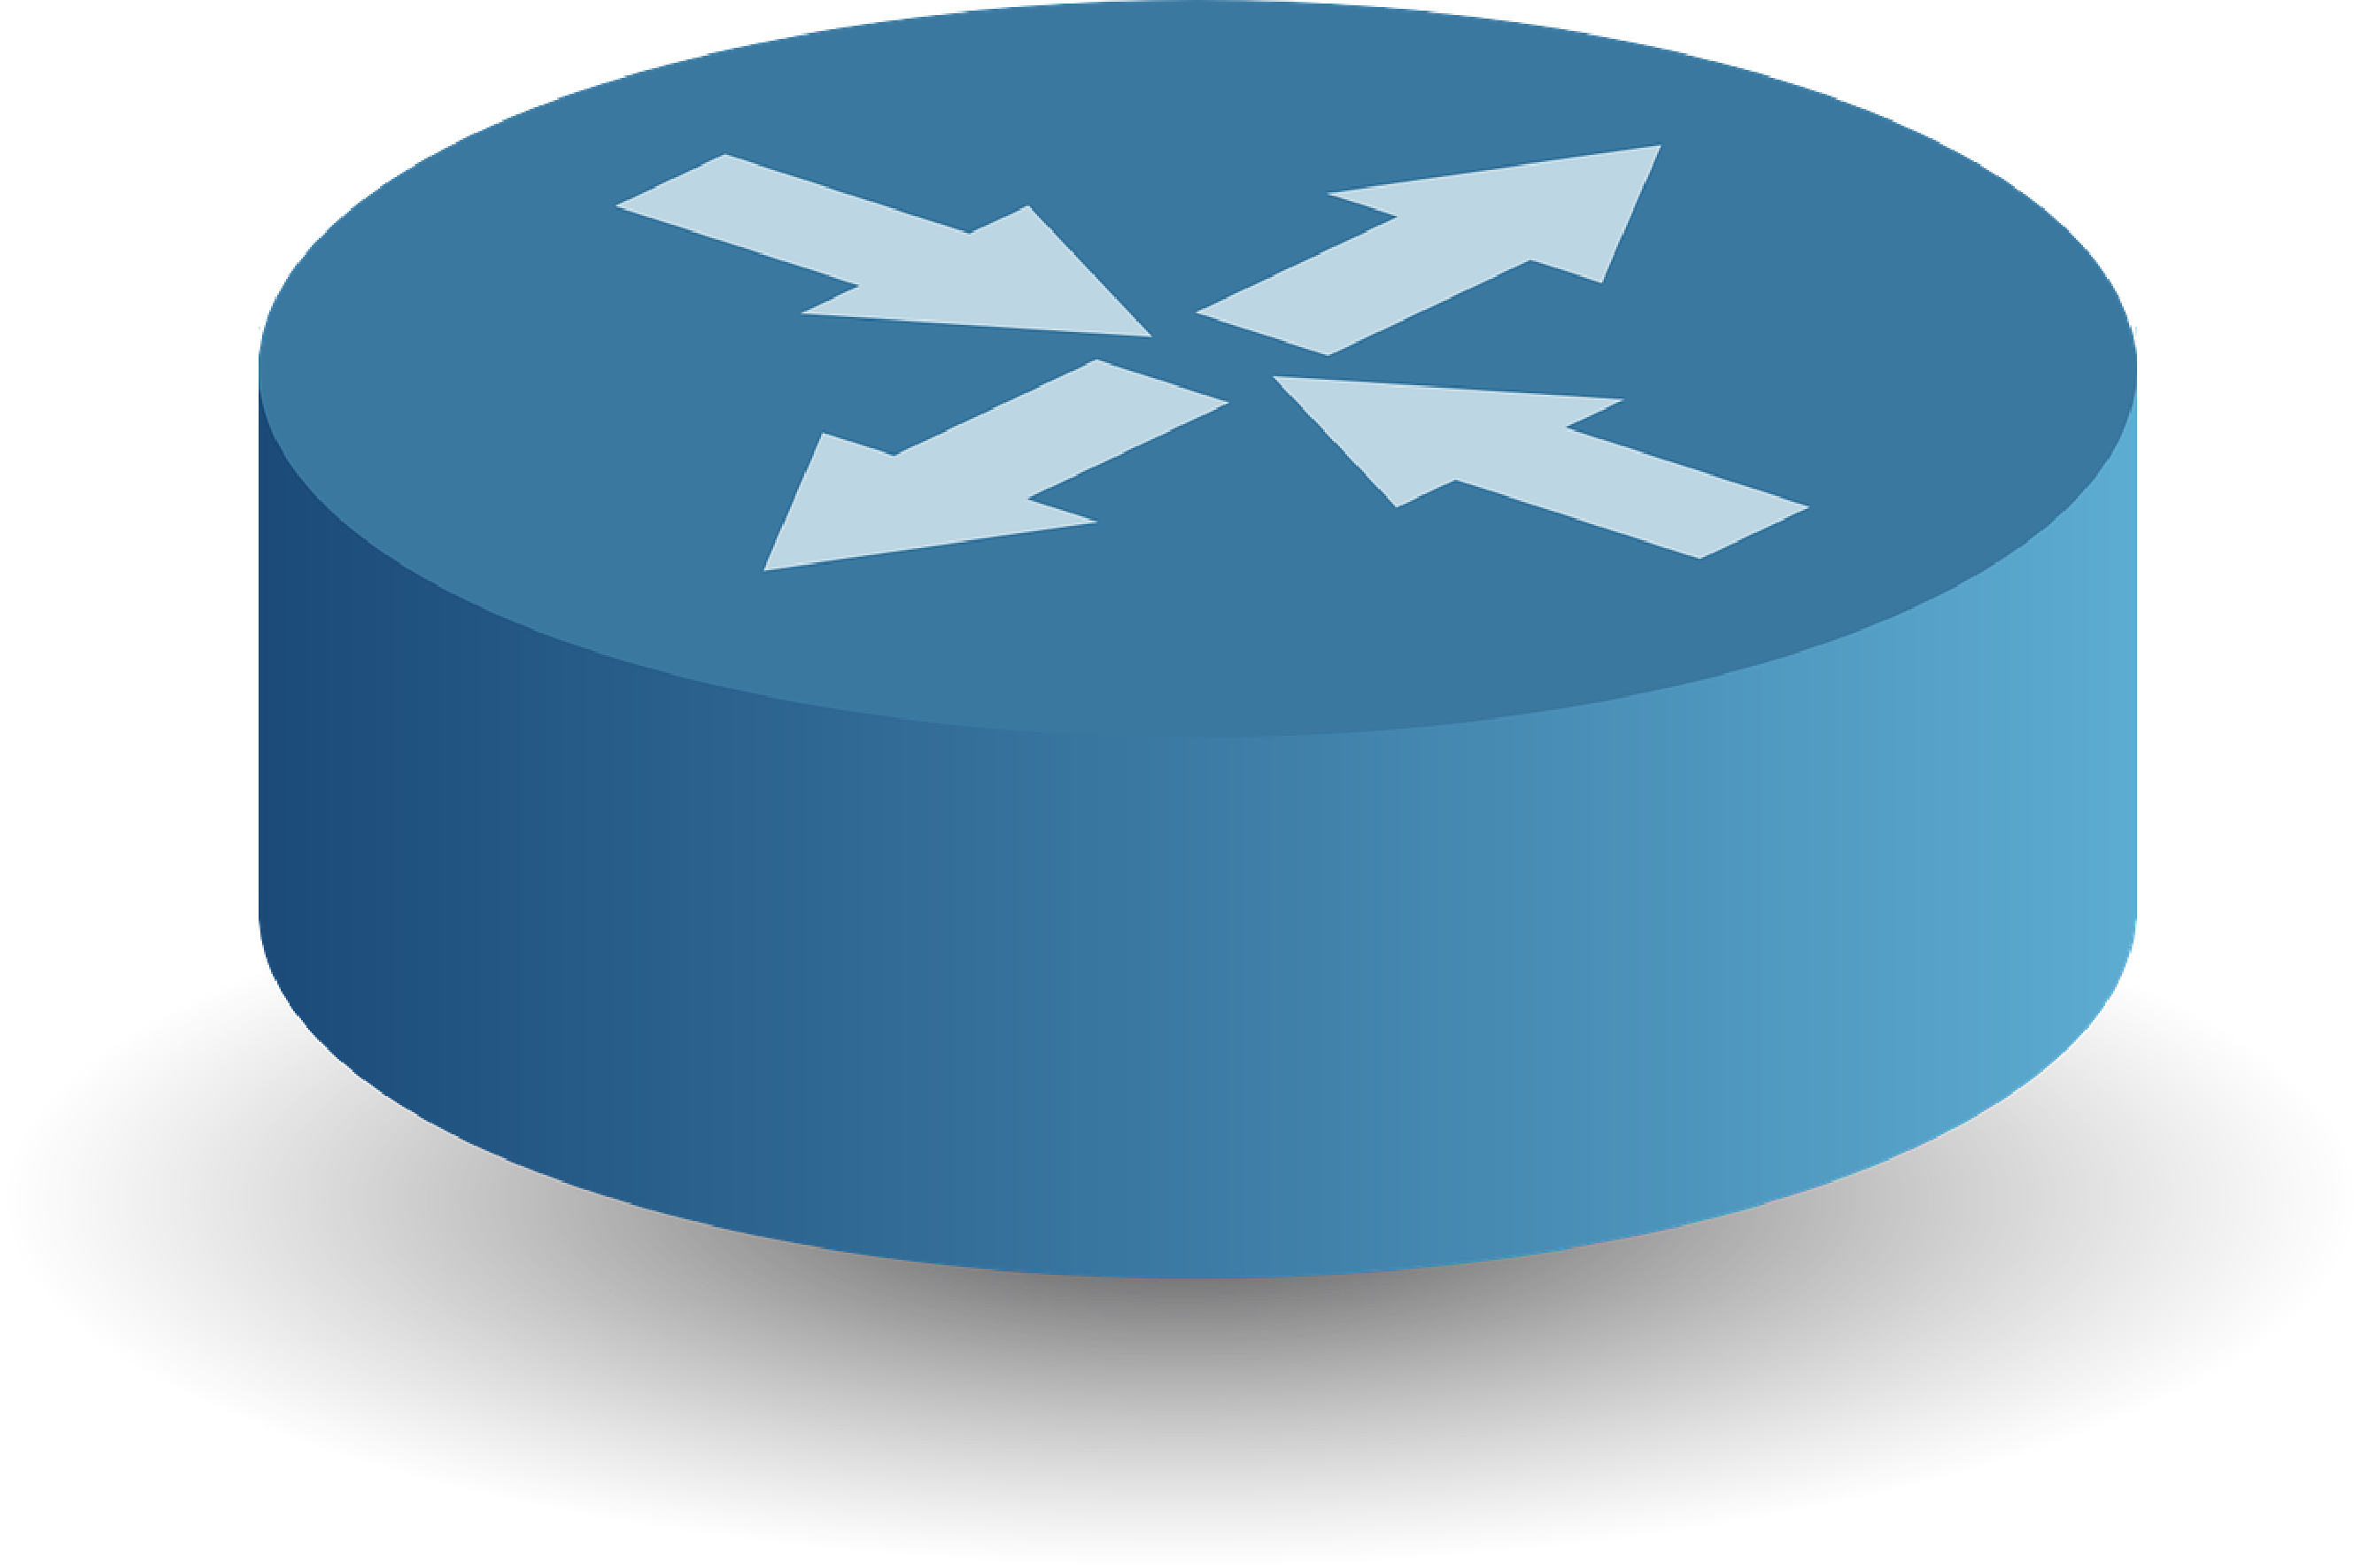
\includegraphics[width=52.5pt,height=52.5pt]{figures/router-29825_1280.pdf}};
%Image [id:dp4786061414756648] 
\draw (248,407.83) node  {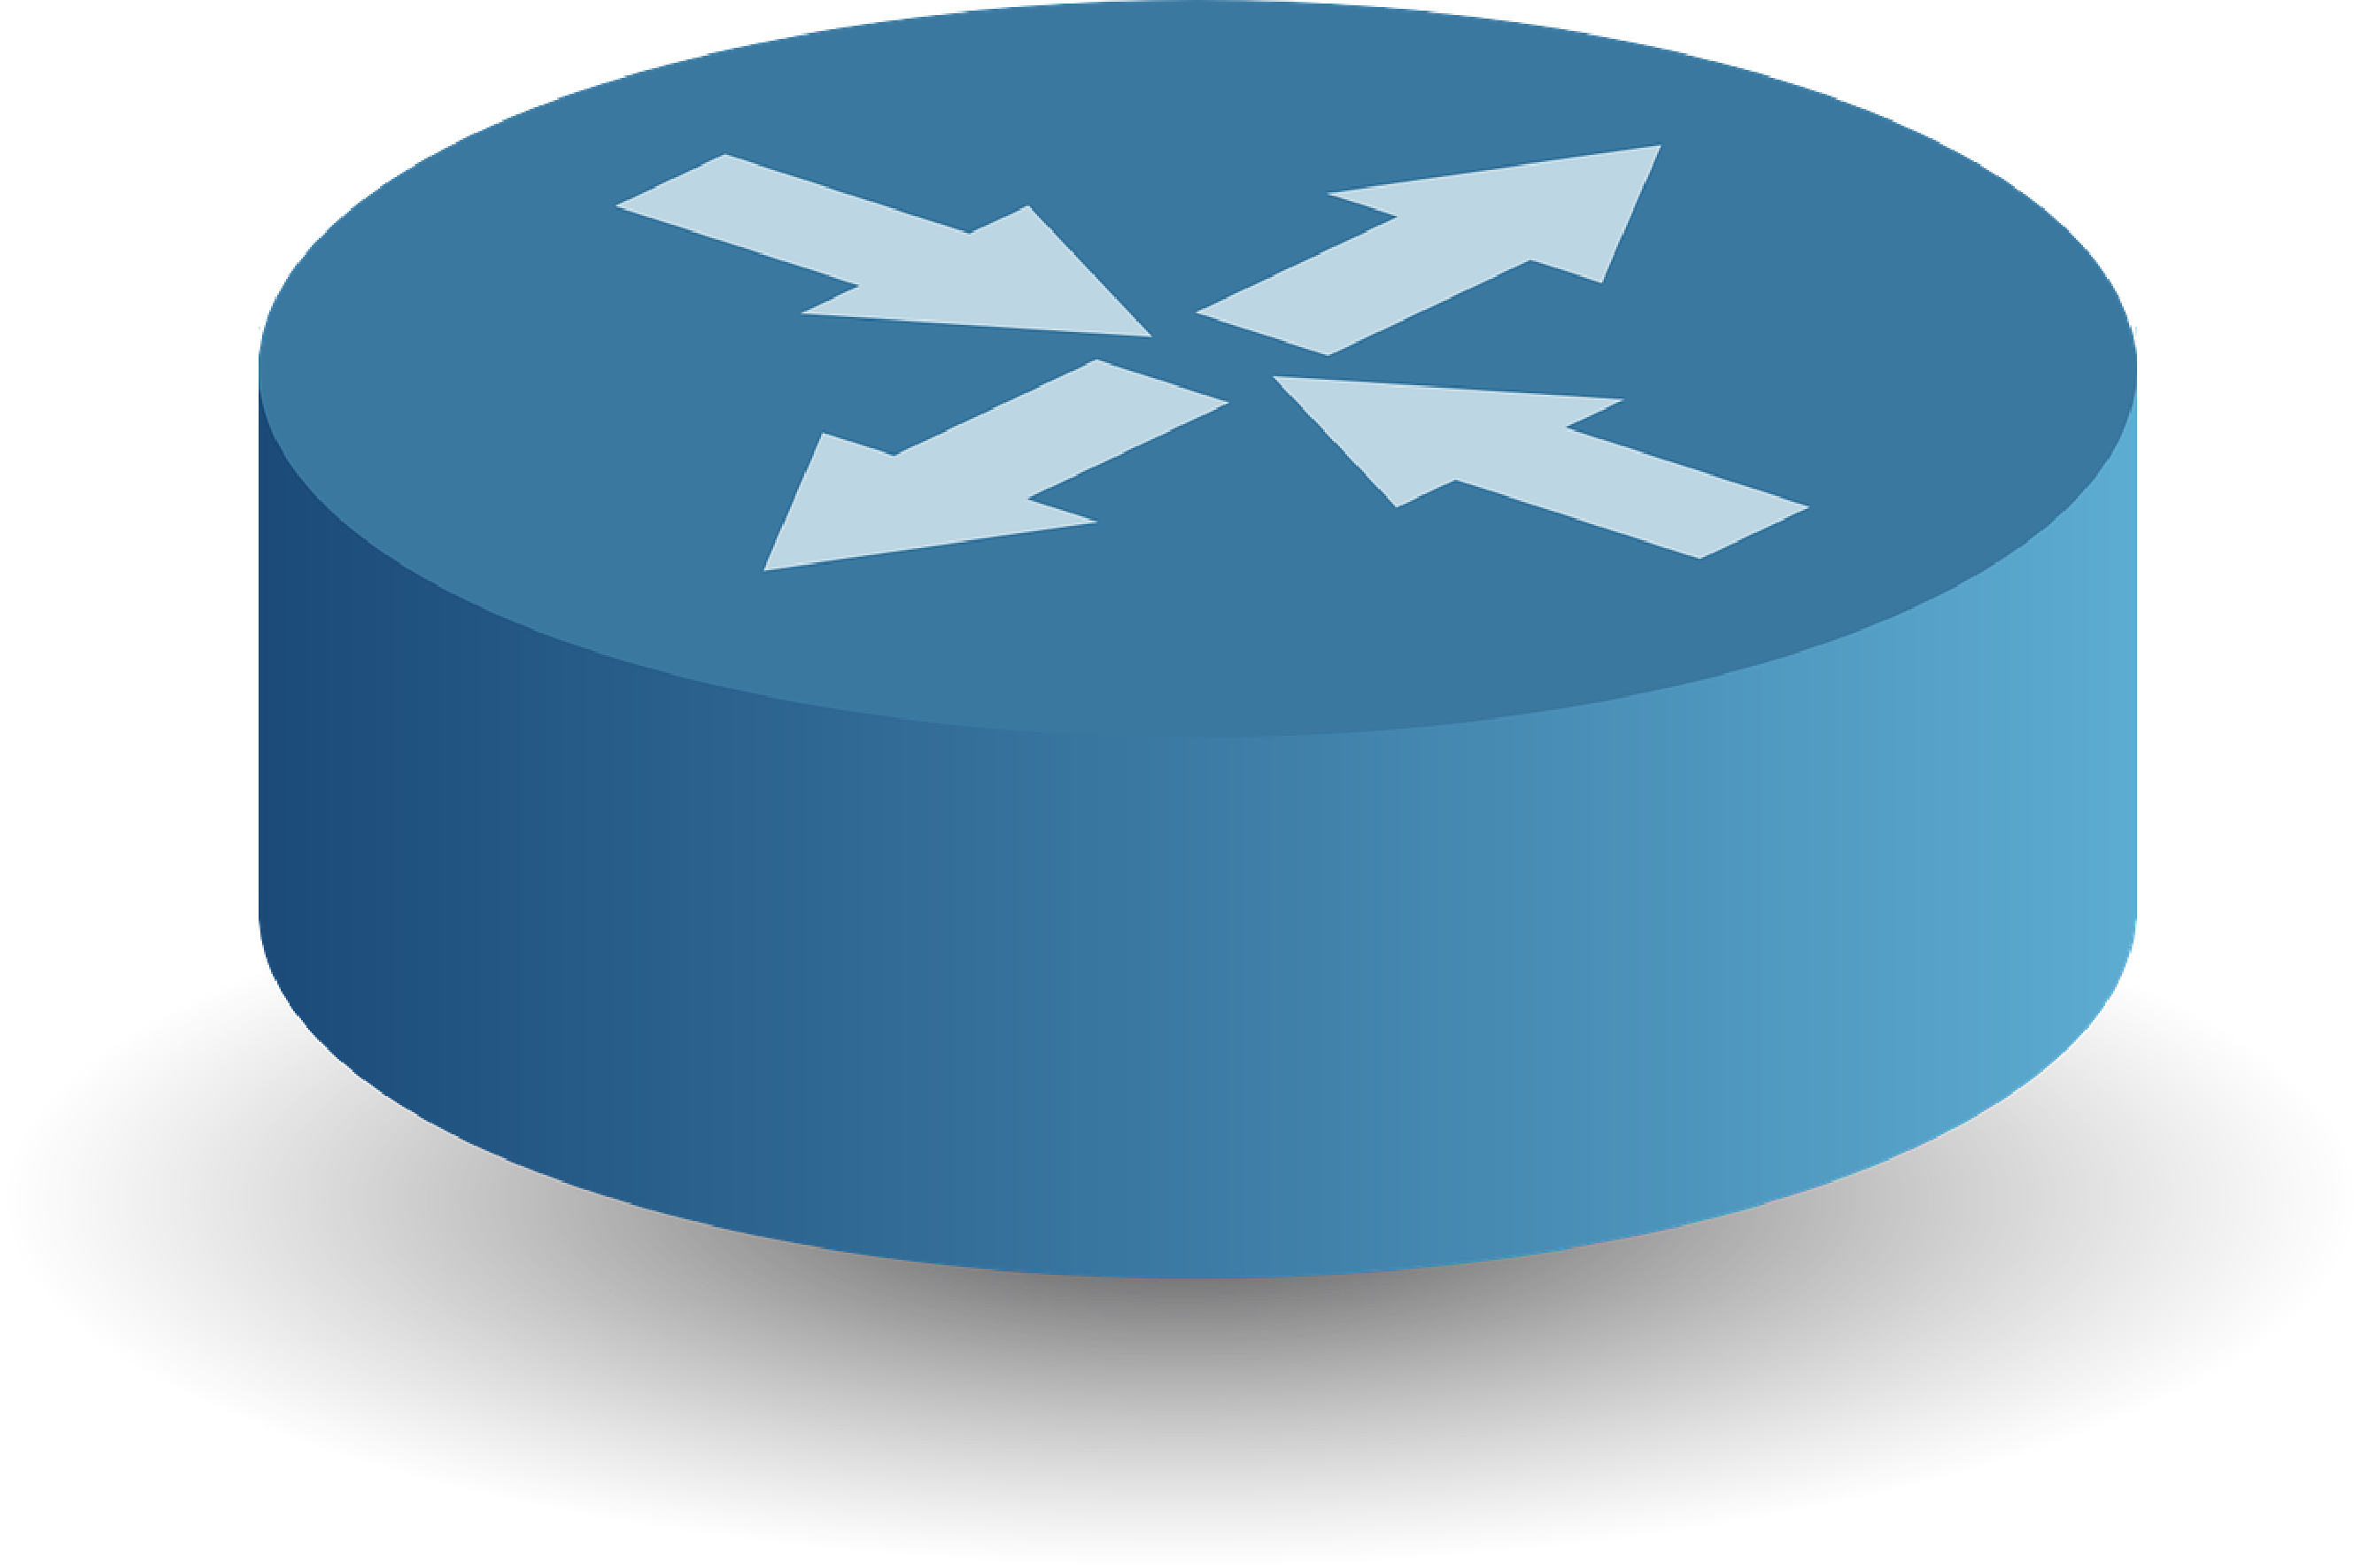
\includegraphics[width=52.5pt,height=52.5pt]{figures/router-29825_1280.pdf}};

%Image [id:dp9691436731399989] 
\draw (365.5,467.83) node  {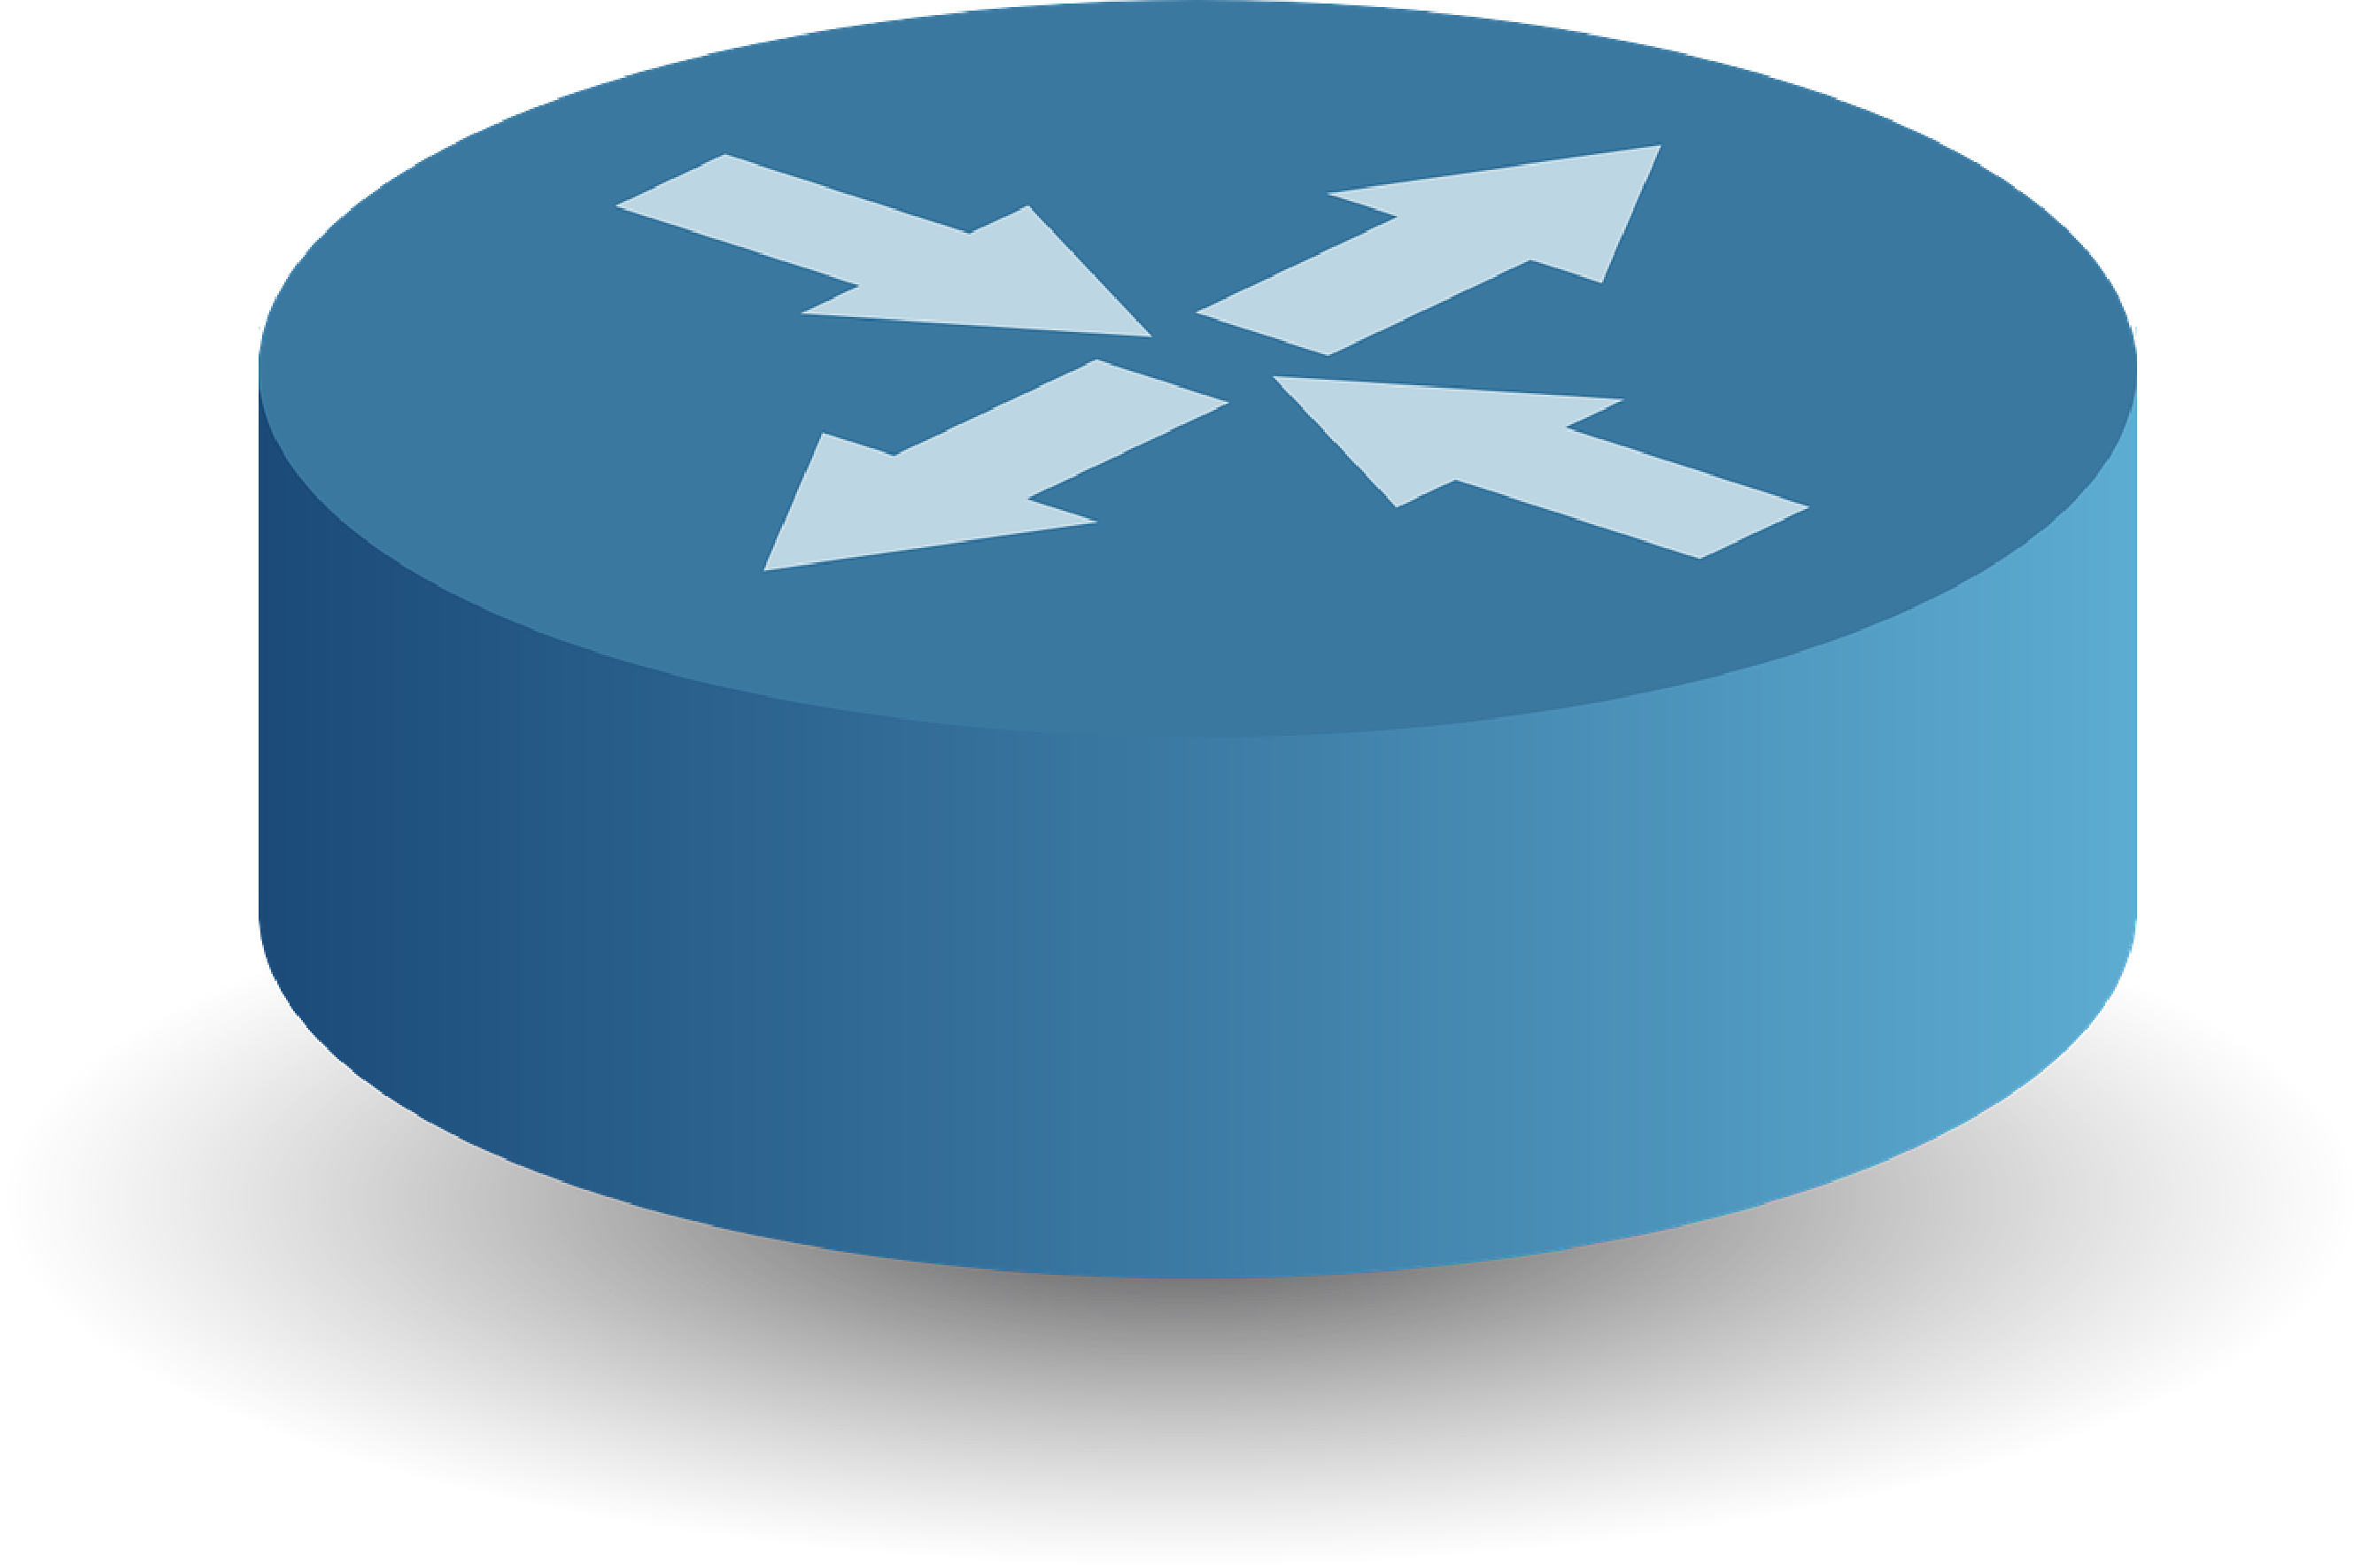
\includegraphics[width=52.5pt,height=52.5pt]{figures/router-29825_1280.pdf}};
%Image [id:dp9494715890151124] 
\draw (130.5,467.83) node  {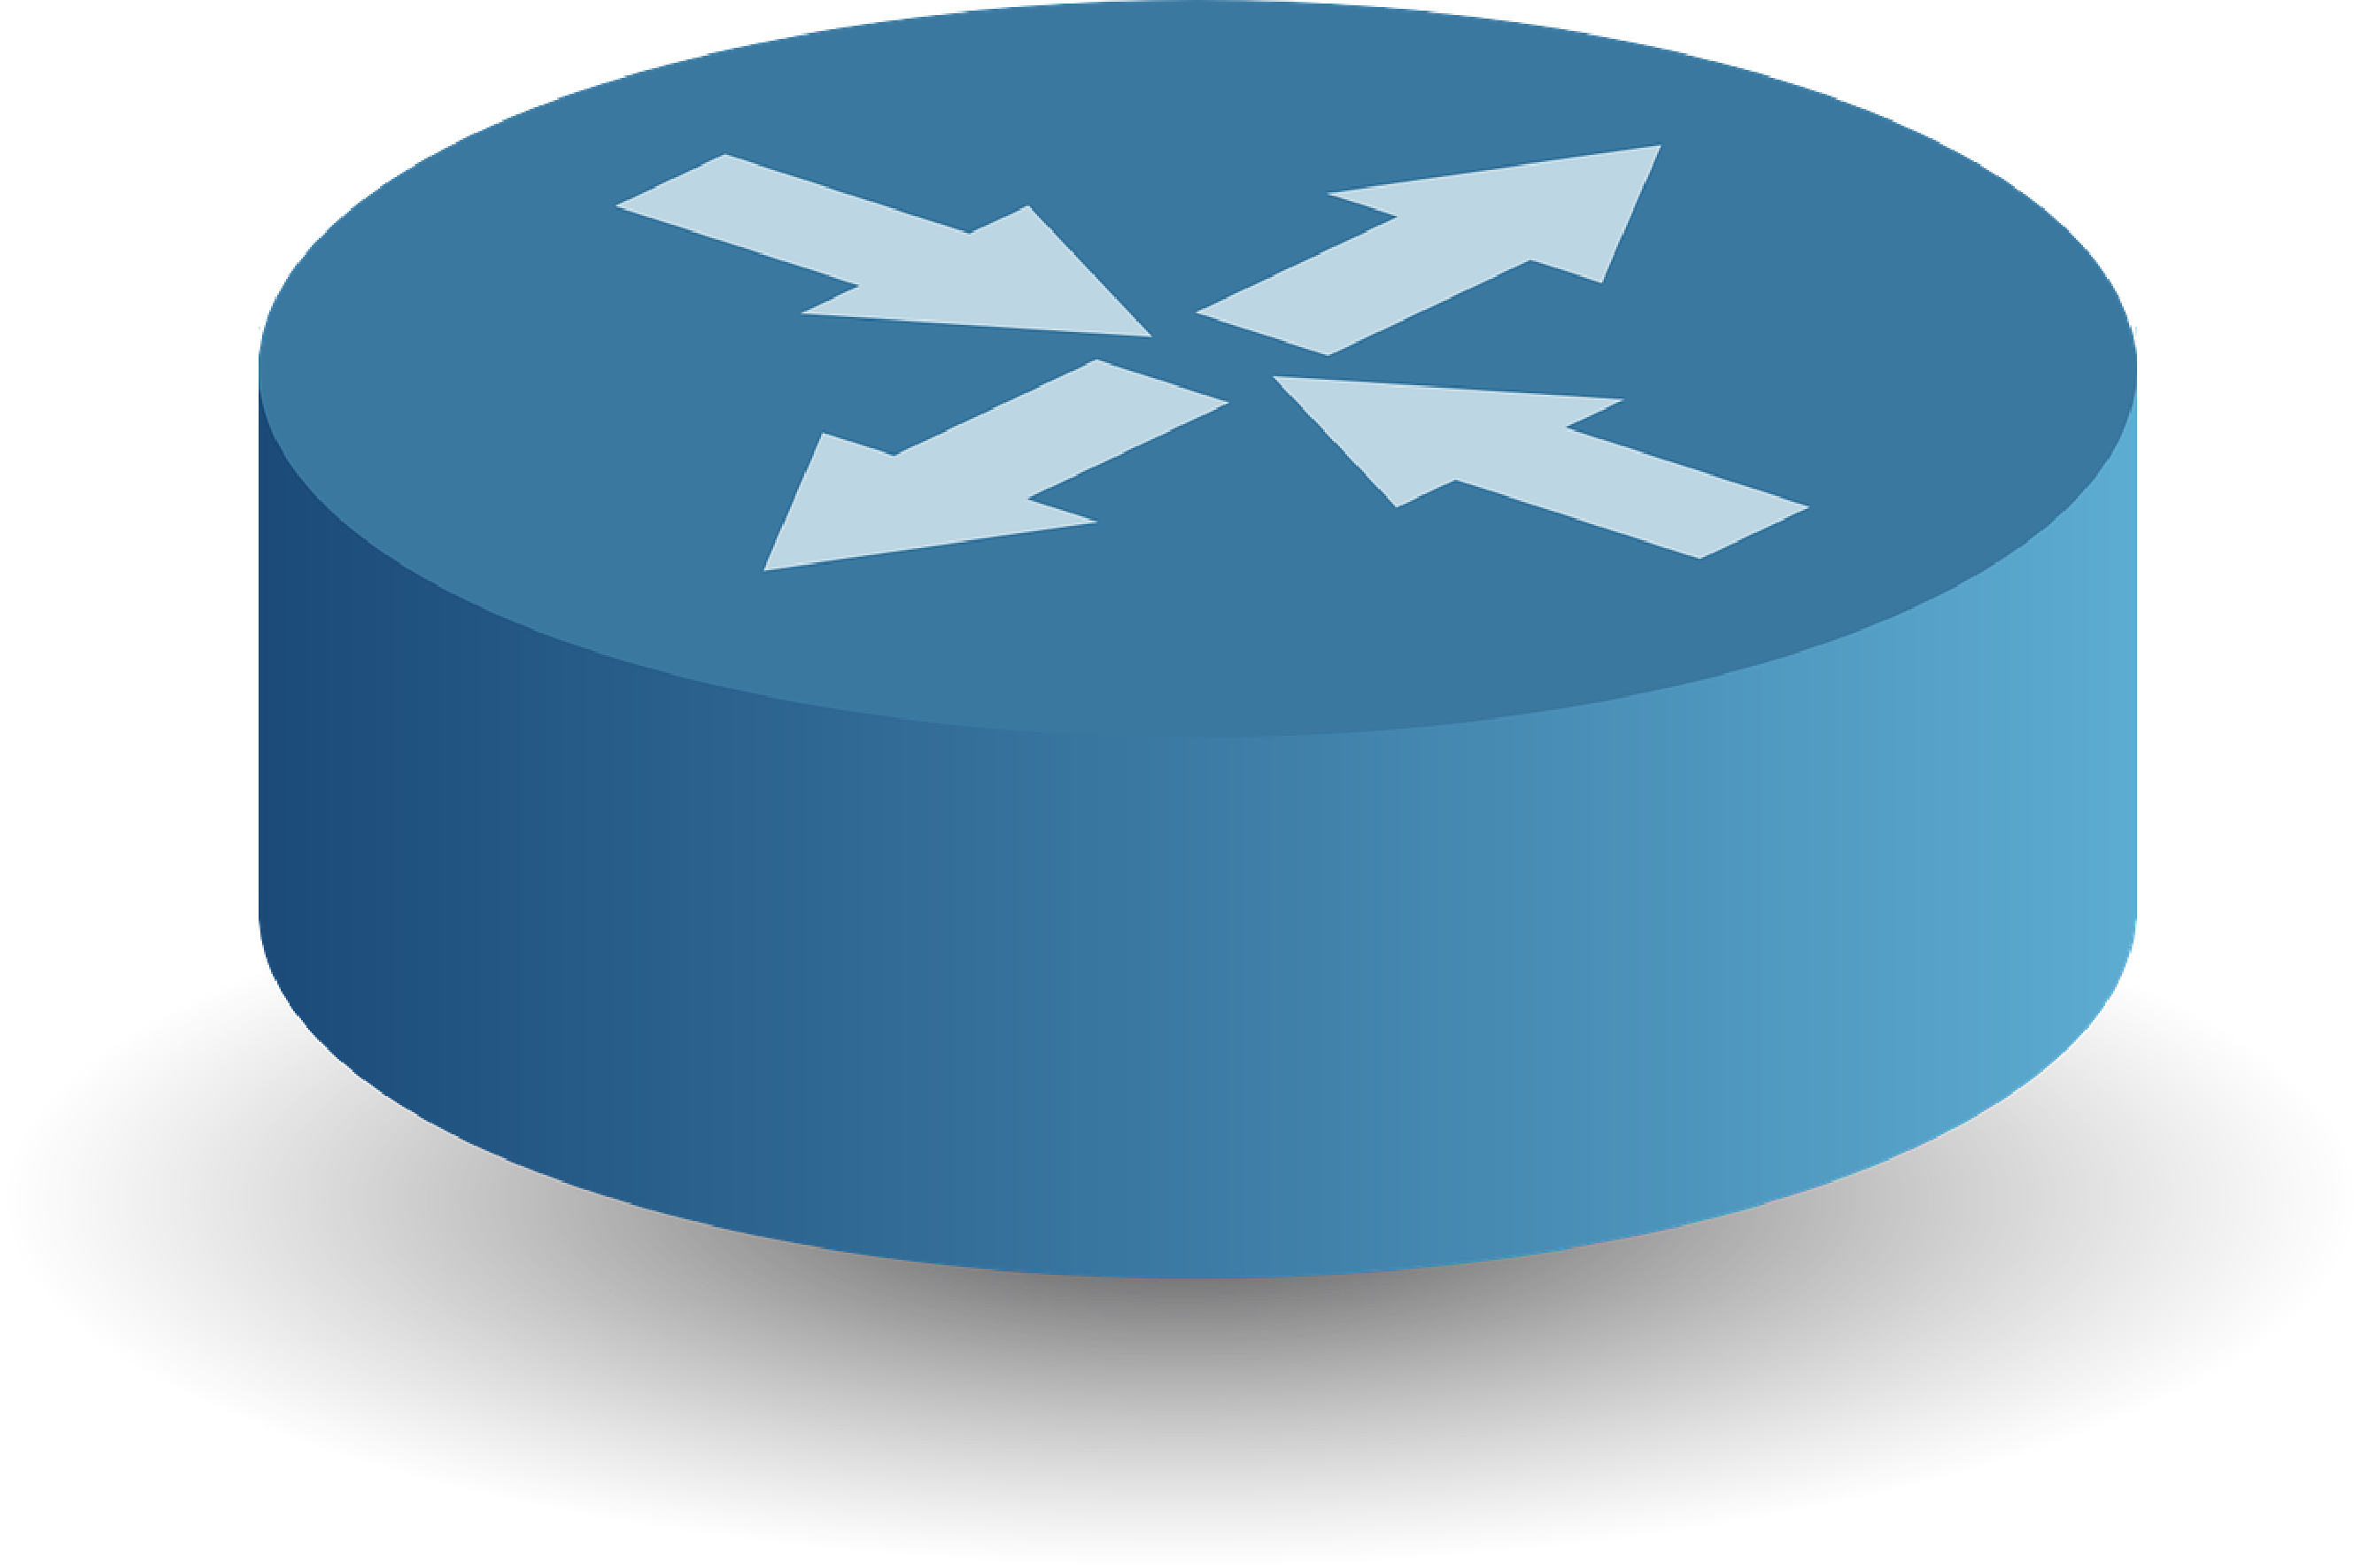
\includegraphics[width=52.5pt,height=52.5pt]{figures/router-29825_1280.pdf}};




%Rounded Rect [id:dp3362169615585995] 
\draw  [fill={rgb, 255:red, 246; green, 185; blue, 255 }  ,fill opacity=1 ] (14.33,161.8) .. controls (14.33,142.3) and (30.14,126.5) .. (49.63,126.5) -- (421.03,126.5) .. controls (440.53,126.5) and (456.33,142.3) .. (456.33,161.8) -- (456.33,267.7) .. controls (456.33,287.2) and (440.53,303) .. (421.03,303) -- (49.63,303) .. controls (30.14,303) and (14.33,287.2) .. (14.33,267.7) -- cycle ;
%Rounded Rect [id:dp9567502407138185] 
\draw  [fill={rgb, 255:red, 255; green, 255; blue, 255 }  ,fill opacity=1 ][line width=1.5]  (210.83,194.22) .. controls (210.83,190.83) and (213.58,188.08) .. (216.97,188.08) -- (310.7,188.08) .. controls (314.09,188.08) and (316.83,190.83) .. (316.83,194.22) -- (316.83,212.62) .. controls (316.83,216) and (314.09,218.75) .. (310.7,218.75) -- (216.97,218.75) .. controls (213.58,218.75) and (210.83,216) .. (210.83,212.62) -- cycle ;

%Rounded Rect [id:dp009214837373342832] 
\draw  [fill={rgb, 255:red, 255; green, 255; blue, 255 }  ,fill opacity=1 ][line width=1.5]  (51.46,194.22) .. controls (51.46,190.83) and (54.2,188.08) .. (57.59,188.08) -- (175.07,188.08) .. controls (178.46,188.08) and (181.21,190.83) .. (181.21,194.22) -- (181.21,212.62) .. controls (181.21,216) and (178.46,218.75) .. (175.07,218.75) -- (57.59,218.75) .. controls (54.2,218.75) and (51.46,216) .. (51.46,212.62) -- cycle ;

%Rounded Rect [id:dp7376385480360085] 
\draw  [fill={rgb, 255:red, 255; green, 255; blue, 255 }  ,fill opacity=1 ][line width=1.5]  (172.05,116.22) .. controls (172.05,112.83) and (174.79,110.08) .. (178.18,110.08) -- (349.49,110.08) .. controls (352.87,110.08) and (355.62,112.83) .. (355.62,116.22) -- (355.62,134.62) .. controls (355.62,138) and (352.87,140.75) .. (349.49,140.75) -- (178.18,140.75) .. controls (174.79,140.75) and (172.05,138) .. (172.05,134.62) -- cycle ;

%Rounded Rect [id:dp19791531901769066] 
\draw  [fill={rgb, 255:red, 255; green, 255; blue, 255 }  ,fill opacity=1 ][line width=1.5]  (172.05,294.22) .. controls (172.05,290.83) and (174.79,288.08) .. (178.18,288.08) -- (349.49,288.08) .. controls (352.87,288.08) and (355.62,290.83) .. (355.62,294.22) -- (355.62,312.62) .. controls (355.62,316) and (352.87,318.75) .. (349.49,318.75) -- (178.18,318.75) .. controls (174.79,318.75) and (172.05,316) .. (172.05,312.62) -- cycle ;

%Straight Lines [id:da3071607162532064] 
\draw  [dash pattern={on 4.5pt off 4.5pt}]  (262.56,144.33) -- (263.44,184.83) ;
\draw [shift={(263.5,187.83)}, rotate = 268.77] [fill={rgb, 255:red, 0; green, 0; blue, 0 }  ][line width=0.08]  [draw opacity=0] (10.72,-5.15) -- (0,0) -- (10.72,5.15) -- (7.12,0) -- cycle    ;
\draw [shift={(262.5,141.33)}, rotate = 88.77] [fill={rgb, 255:red, 0; green, 0; blue, 0 }  ][line width=0.08]  [draw opacity=0] (10.72,-5.15) -- (0,0) -- (10.72,5.15) -- (7.12,0) -- cycle    ;
%Straight Lines [id:da5811563165265446] 
\draw  [dash pattern={on 4.5pt off 4.5pt}]  (120.06,239.8) -- (119.14,220.83) ;
\draw [shift={(119,217.83)}, rotate = 447.25] [fill={rgb, 255:red, 0; green, 0; blue, 0 }  ][line width=0.08]  [draw opacity=0] (10.72,-5.15) -- (0,0) -- (10.72,5.15) -- (7.12,0) -- cycle    ;
\draw [shift={(120.2,242.8)}, rotate = 267.25] [fill={rgb, 255:red, 0; green, 0; blue, 0 }  ][line width=0.08]  [draw opacity=0] (10.72,-5.15) -- (0,0) -- (10.72,5.15) -- (7.12,0) -- cycle    ;
%Straight Lines [id:da36813314079504633] 
\draw  [dash pattern={on 4.5pt off 4.5pt}]  (189,250) -- (209.32,215.21) ;
\draw [shift={(210.83,212.62)}, rotate = 480.29] [fill={rgb, 255:red, 0; green, 0; blue, 0 }  ][line width=0.08]  [draw opacity=0] (10.72,-5.15) -- (0,0) -- (10.72,5.15) -- (7.12,0) -- cycle    ;

%Straight Lines [id:da7736079542900215] 
\draw  [dash pattern={on 4.5pt off 4.5pt}]  (263,222.83) -- (263,284.83) ;
\draw [shift={(263,287.83)}, rotate = 270] [fill={rgb, 255:red, 0; green, 0; blue, 0 }  ][line width=0.08]  [draw opacity=0] (10.72,-5.15) -- (0,0) -- (10.72,5.15) -- (7.12,0) -- cycle    ;
\draw [shift={(263,219.83)}, rotate = 90] [fill={rgb, 255:red, 0; green, 0; blue, 0 }  ][line width=0.08]  [draw opacity=0] (10.72,-5.15) -- (0,0) -- (10.72,5.15) -- (7.12,0) -- cycle    ;
%Straight Lines [id:da5692634255089728] 
\draw  [dash pattern={on 4.5pt off 4.5pt}]  (185,204.23) -- (207,203.44) ;
\draw [shift={(210,203.33)}, rotate = 537.95] [fill={rgb, 255:red, 0; green, 0; blue, 0 }  ][line width=0.08]  [draw opacity=0] (10.72,-5.15) -- (0,0) -- (10.72,5.15) -- (7.12,0) -- cycle    ;
\draw [shift={(182,204.33)}, rotate = 357.95] [fill={rgb, 255:red, 0; green, 0; blue, 0 }  ][line width=0.08]  [draw opacity=0] (10.72,-5.15) -- (0,0) -- (10.72,5.15) -- (7.12,0) -- cycle    ;
%Straight Lines [id:da11917773489604144] 
\draw  [dash pattern={on 4.5pt off 4.5pt}]  (195.8,259.02) -- (328.77,256.62) ;
\draw [shift={(331.77,256.57)}, rotate = 538.97] [fill={rgb, 255:red, 0; green, 0; blue, 0 }  ][line width=0.08]  [draw opacity=0] (10.72,-5.15) -- (0,0) -- (10.72,5.15) -- (7.12,0) -- cycle    ;

%Straight Lines [id:da7770404819607903] 
\draw  [dash pattern={on 4.5pt off 4.5pt}]  (262.81,322.31) -- (262.98,351.33) ;
\draw [shift={(263,354.33)}, rotate = 269.65999999999997] [fill={rgb, 255:red, 0; green, 0; blue, 0 }  ][line width=0.08]  [draw opacity=0] (10.72,-5.15) -- (0,0) -- (10.72,5.15) -- (7.12,0) -- cycle    ;
\draw [shift={(262.79,319.31)}, rotate = 89.66] [fill={rgb, 255:red, 0; green, 0; blue, 0 }  ][line width=0.08]  [draw opacity=0] (10.72,-5.15) -- (0,0) -- (10.72,5.15) -- (7.12,0) -- cycle    ;
%Straight Lines [id:da8379163771385384] 
\draw  [dash pattern={on 4.5pt off 4.5pt}]  (145.98,273.33) -- (145.46,349.78) ;
\draw [shift={(145.44,352.78)}, rotate = 270.39] [fill={rgb, 255:red, 0; green, 0; blue, 0 }  ][line width=0.08]  [draw opacity=0] (10.72,-5.15) -- (0,0) -- (10.72,5.15) -- (7.12,0) -- cycle    ;
\draw [shift={(146,270.33)}, rotate = 90.39] [fill={rgb, 255:red, 0; green, 0; blue, 0 }  ][line width=0.08]  [draw opacity=0] (10.72,-5.15) -- (0,0) -- (10.72,5.15) -- (7.12,0) -- cycle    ;
%Straight Lines [id:da7179548819350594] 
\draw  [dash pattern={on 4.5pt off 4.5pt}]  (263,72.33) -- (263,106.33) ;
\draw [shift={(263,109.33)}, rotate = 270] [fill={rgb, 255:red, 0; green, 0; blue, 0 }  ][line width=0.08]  [draw opacity=0] (10.72,-5.15) -- (0,0) -- (10.72,5.15) -- (7.12,0) -- cycle    ;
\draw [shift={(263,69.33)}, rotate = 90] [fill={rgb, 255:red, 0; green, 0; blue, 0 }  ][line width=0.08]  [draw opacity=0] (10.72,-5.15) -- (0,0) -- (10.72,5.15) -- (7.12,0) -- cycle    ;
%Rounded Rect [id:dp3518984914276363] 
\draw  [fill={rgb, 255:red, 56; green, 144; blue, 249 }  ,fill opacity=1 ] (121.5,17.37) .. controls (121.5,9.98) and (127.48,4) .. (134.87,4) -- (361.13,4) .. controls (368.52,4) and (374.5,9.98) .. (374.5,17.37) -- (374.5,57.47) .. controls (374.5,64.85) and (368.52,70.83) .. (361.13,70.83) -- (134.87,70.83) .. controls (127.48,70.83) and (121.5,64.85) .. (121.5,57.47) -- cycle ;
%Rounded Rect [id:dp09188382569915587] 
\draw  [color={rgb, 255:red, 0; green, 0; blue, 0 }  ,draw opacity=1 ][fill={rgb, 255:red, 255; green, 255; blue, 255 }  ,fill opacity=1 ][dash pattern={on 5.63pt off 4.5pt}][line width=1.5]  (129.7,35.2) .. controls (129.7,31.87) and (132.4,29.17) .. (135.73,29.17) -- (234.94,29.17) .. controls (238.27,29.17) and (240.97,31.87) .. (240.97,35.2) -- (240.97,53.3) .. controls (240.97,56.63) and (238.27,59.33) .. (234.94,59.33) -- (135.73,59.33) .. controls (132.4,59.33) and (129.7,56.63) .. (129.7,53.3) -- cycle ;
%Rounded Rect [id:dp24603064281963627] 
\draw  [color={rgb, 255:red, 0; green, 0; blue, 0 }  ,draw opacity=1 ][fill={rgb, 255:red, 255; green, 255; blue, 255 }  ,fill opacity=1 ][dash pattern={on 5.63pt off 4.5pt}][line width=1.5]  (255.03,35.2) .. controls (255.03,31.87) and (257.73,29.17) .. (261.06,29.17) -- (360.27,29.17) .. controls (363.6,29.17) and (366.3,31.87) .. (366.3,35.2) -- (366.3,53.3) .. controls (366.3,56.63) and (363.6,59.33) .. (360.27,59.33) -- (261.06,59.33) .. controls (257.73,59.33) and (255.03,56.63) .. (255.03,53.3) -- cycle ;

%Rounded Rect [id:dp758697930562836] 
\draw  [fill={rgb, 255:red, 255; green, 255; blue, 255 }  ,fill opacity=1 ][line width=1.5]  (109.06,245.55) .. controls (109.06,242.16) and (111.81,239.42) .. (115.19,239.42) -- (191.47,239.42) .. controls (194.86,239.42) and (197.6,242.16) .. (197.6,245.55) -- (197.6,263.95) .. controls (197.6,267.34) and (194.86,270.08) .. (191.47,270.08) -- (115.19,270.08) .. controls (111.81,270.08) and (109.06,267.34) .. (109.06,263.95) -- cycle ;

%Straight Lines [id:da6795518551939627] 
\draw  [dash pattern={on 4.5pt off 4.5pt}]  (325,143.83) -- (324.78,284.78) ;
\draw [shift={(324.78,287.78)}, rotate = 270.09000000000003] [fill={rgb, 255:red, 0; green, 0; blue, 0 }  ][line width=0.08]  [draw opacity=0] (10.72,-5.15) -- (0,0) -- (10.72,5.15) -- (7.12,0) -- cycle    ;
\draw [shift={(325,140.83)}, rotate = 90.09] [fill={rgb, 255:red, 0; green, 0; blue, 0 }  ][line width=0.08]  [draw opacity=0] (10.72,-5.15) -- (0,0) -- (10.72,5.15) -- (7.12,0) -- cycle    ;
%Straight Lines [id:da055910518428688105] 
\draw  [dash pattern={on 4.5pt off 4.5pt}]  (185.78,140.44) -- (185.72,236.92) ;
\draw [shift={(185.72,239.92)}, rotate = 270.03] [fill={rgb, 255:red, 0; green, 0; blue, 0 }  ][line width=0.08]  [draw opacity=0] (10.72,-5.15) -- (0,0) -- (10.72,5.15) -- (7.12,0) -- cycle    ;

%Straight Lines [id:da9613526114203358] 
\draw  [dash pattern={on 4.5pt off 4.5pt}]  (66.42,221.44) -- (65.78,295.78) -- (169.05,294.26) ;
\draw [shift={(172.05,294.22)}, rotate = 539.1600000000001] [fill={rgb, 255:red, 0; green, 0; blue, 0 }  ][line width=0.08]  [draw opacity=0] (10.72,-5.15) -- (0,0) -- (10.72,5.15) -- (7.12,0) -- cycle    ;
\draw [shift={(66.44,218.44)}, rotate = 90.49] [fill={rgb, 255:red, 0; green, 0; blue, 0 }  ][line width=0.08]  [draw opacity=0] (10.72,-5.15) -- (0,0) -- (10.72,5.15) -- (7.12,0) -- cycle    ;
%Straight Lines [id:da3742893196331808] 
\draw  [dash pattern={on 4.5pt off 4.5pt}]  (348.07,143.83) -- (350.1,234.17) ;
\draw [shift={(350.17,237.17)}, rotate = 268.71] [fill={rgb, 255:red, 0; green, 0; blue, 0 }  ][line width=0.08]  [draw opacity=0] (10.72,-5.15) -- (0,0) -- (10.72,5.15) -- (7.12,0) -- cycle    ;
\draw [shift={(348,140.83)}, rotate = 88.71] [fill={rgb, 255:red, 0; green, 0; blue, 0 }  ][line width=0.08]  [draw opacity=0] (10.72,-5.15) -- (0,0) -- (10.72,5.15) -- (7.12,0) -- cycle    ;
%Rounded Rect [id:dp9140860086605985] 
\draw  [fill={rgb, 255:red, 255; green, 255; blue, 255 }  ,fill opacity=1 ][line width=1.5]  (335.83,245.55) .. controls (335.83,242.16) and (338.58,239.42) .. (341.97,239.42) -- (435.7,239.42) .. controls (439.09,239.42) and (441.83,242.16) .. (441.83,245.55) -- (441.83,263.95) .. controls (441.83,267.34) and (439.09,270.08) .. (435.7,270.08) -- (341.97,270.08) .. controls (338.58,270.08) and (335.83,267.34) .. (335.83,263.95) -- cycle ;

%Shape: Ellipse [id:dp3554083551130477] 
\draw  [color={rgb, 255:red, 208; green, 2; blue, 27 }  ,draw opacity=1 ] (188.3,153.75) .. controls (188.3,149.91) and (191.71,146.8) .. (195.93,146.8) .. controls (200.14,146.8) and (203.55,149.91) .. (203.55,153.75) .. controls (203.55,157.59) and (200.14,160.7) .. (195.93,160.7) .. controls (191.71,160.7) and (188.3,157.59) .. (188.3,153.75) -- cycle ;
%Shape: Ellipse [id:dp4084549692042517] 
\draw  [color={rgb, 255:red, 208; green, 2; blue, 27 }  ,draw opacity=1 ] (267.05,87.25) .. controls (267.05,83.41) and (270.46,80.3) .. (274.68,80.3) .. controls (278.89,80.3) and (282.3,83.41) .. (282.3,87.25) .. controls (282.3,91.09) and (278.89,94.2) .. (274.68,94.2) .. controls (270.46,94.2) and (267.05,91.09) .. (267.05,87.25) -- cycle ;
%Shape: Ellipse [id:dp6652927550013479] 
\draw  [color={rgb, 255:red, 208; green, 2; blue, 27 }  ,draw opacity=1 ] (264.8,156.5) .. controls (264.8,152.66) and (268.21,149.55) .. (272.43,149.55) .. controls (276.64,149.55) and (280.05,152.66) .. (280.05,156.5) .. controls (280.05,160.34) and (276.64,163.45) .. (272.43,163.45) .. controls (268.21,163.45) and (264.8,160.34) .. (264.8,156.5) -- cycle ;
%Shape: Ellipse [id:dp20966000134493123] 
\draw  [color={rgb, 255:red, 208; green, 2; blue, 27 }  ,draw opacity=1 ] (307.55,151.25) .. controls (307.55,147.41) and (310.96,144.3) .. (315.18,144.3) .. controls (319.39,144.3) and (322.8,147.41) .. (322.8,151.25) .. controls (322.8,155.09) and (319.39,158.2) .. (315.18,158.2) .. controls (310.96,158.2) and (307.55,155.09) .. (307.55,151.25) -- cycle ;
%Shape: Ellipse [id:dp0540432112177649] 
\draw  [color={rgb, 255:red, 208; green, 2; blue, 27 }  ,draw opacity=1 ] (355.55,180.75) .. controls (355.55,176.91) and (358.96,173.8) .. (363.18,173.8) .. controls (367.39,173.8) and (370.8,176.91) .. (370.8,180.75) .. controls (370.8,184.59) and (367.39,187.7) .. (363.18,187.7) .. controls (358.96,187.7) and (355.55,184.59) .. (355.55,180.75) -- cycle ;
%Shape: Ellipse [id:dp45917488569940357] 
\draw  [color={rgb, 255:red, 208; green, 2; blue, 27 }  ,draw opacity=1 ] (185.3,189.34) .. controls (185.3,185.5) and (188.71,182.39) .. (192.93,182.39) .. controls (197.14,182.39) and (200.55,185.5) .. (200.55,189.34) .. controls (200.55,193.17) and (197.14,196.28) .. (192.93,196.28) .. controls (188.71,196.28) and (185.3,193.17) .. (185.3,189.34) -- cycle ;

%Shape: Ellipse [id:dp5545246337247209] 
\draw  [color={rgb, 255:red, 208; green, 2; blue, 27 }  ,draw opacity=1 ] (199.3,229) .. controls (199.3,225.16) and (202.71,222.05) .. (206.93,222.05) .. controls (211.14,222.05) and (214.55,225.16) .. (214.55,229) .. controls (214.55,232.84) and (211.14,235.95) .. (206.93,235.95) .. controls (202.71,235.95) and (199.3,232.84) .. (199.3,229) -- cycle ;
%Shape: Ellipse [id:dp4152293630769399] 
\draw  [color={rgb, 255:red, 208; green, 2; blue, 27 }  ,draw opacity=1 ] (264.1,229.6) .. controls (264.1,225.76) and (267.51,222.65) .. (271.73,222.65) .. controls (275.94,222.65) and (279.35,225.76) .. (279.35,229.6) .. controls (279.35,233.44) and (275.94,236.55) .. (271.73,236.55) .. controls (267.51,236.55) and (264.1,233.44) .. (264.1,229.6) -- cycle ;
%Shape: Ellipse [id:dp7028700683432993] 
\draw  [color={rgb, 255:red, 208; green, 2; blue, 27 }  ,draw opacity=1 ] (230.1,249.27) .. controls (230.1,245.43) and (233.51,242.32) .. (237.73,242.32) .. controls (241.94,242.32) and (245.35,245.43) .. (245.35,249.27) .. controls (245.35,253.11) and (241.94,256.22) .. (237.73,256.22) .. controls (233.51,256.22) and (230.1,253.11) .. (230.1,249.27) -- cycle ;
%Shape: Ellipse [id:dp07410075663096749] 
\draw  [color={rgb, 255:red, 208; green, 2; blue, 27 }  ,draw opacity=1 ] (121.1,228.62) .. controls (121.1,224.05) and (125.15,220.35) .. (130.15,220.35) .. controls (135.15,220.35) and (139.2,224.05) .. (139.2,228.62) .. controls (139.2,233.18) and (135.15,236.88) .. (130.15,236.88) .. controls (125.15,236.88) and (121.1,233.18) .. (121.1,228.62) -- cycle ;
%Shape: Ellipse [id:dp30224928873301715] 
\draw  [color={rgb, 255:red, 208; green, 2; blue, 27 }  ,draw opacity=1 ] (68.3,284.22) .. controls (68.3,279.65) and (72.35,275.95) .. (77.35,275.95) .. controls (82.35,275.95) and (86.4,279.65) .. (86.4,284.22) .. controls (86.4,288.78) and (82.35,292.48) .. (77.35,292.48) .. controls (72.35,292.48) and (68.3,288.78) .. (68.3,284.22) -- cycle ;
%Shape: Ellipse [id:dp3894329820493001] 
\draw  [color={rgb, 255:red, 208; green, 2; blue, 27 }  ,draw opacity=1 ] (149.5,280.62) .. controls (149.5,276.05) and (153.55,272.35) .. (158.55,272.35) .. controls (163.55,272.35) and (167.6,276.05) .. (167.6,280.62) .. controls (167.6,285.18) and (163.55,288.88) .. (158.55,288.88) .. controls (153.55,288.88) and (149.5,285.18) .. (149.5,280.62) -- cycle ;
%Shape: Ellipse [id:dp8973642196115625] 
\draw  [color={rgb, 255:red, 208; green, 2; blue, 27 }  ,draw opacity=1 ] (375.5,281.22) .. controls (375.5,276.65) and (379.55,272.95) .. (384.55,272.95) .. controls (389.55,272.95) and (393.6,276.65) .. (393.6,281.22) .. controls (393.6,285.78) and (389.55,289.48) .. (384.55,289.48) .. controls (379.55,289.48) and (375.5,285.78) .. (375.5,281.22) -- cycle ;
%Shape: Ellipse [id:dp6431628695495194] 
\draw  [color={rgb, 255:red, 208; green, 2; blue, 27 }  ,draw opacity=1 ] (265.5,335.02) .. controls (265.5,330.45) and (269.55,326.75) .. (274.55,326.75) .. controls (279.55,326.75) and (283.6,330.45) .. (283.6,335.02) .. controls (283.6,339.58) and (279.55,343.28) .. (274.55,343.28) .. controls (269.55,343.28) and (265.5,339.58) .. (265.5,335.02) -- cycle ;
%Straight Lines [id:da6717664493405898] 
\draw  [dash pattern={on 4.5pt off 4.5pt}]  (404.17,275.17) -- (404.17,293.17) -- (355.62,294.22) ;

\draw [shift={(404.17,272.17)}, rotate = 90] [fill={rgb, 255:red, 0; green, 0; blue, 0 }  ][line width=0.08]  [draw opacity=0] (10.72,-5.15) -- (0,0) -- (10.72,5.15) -- (7.12,0) -- cycle    ;

% Text Node
\draw (106.66,137.09) node  [font=\small] [align=left] {Network Hypervisor};
% Text Node
\draw (196.26,154.45) node  [color={rgb, 255:red, 208; green, 2; blue, 27 }  ,opacity=1 ] [align=left] {3};
% Text Node
\draw (275.01,86.95) node  [color={rgb, 255:red, 208; green, 2; blue, 27 }  ,opacity=1 ] [align=left] {1};
% Text Node
\draw (272.76,157.2) node  [font=\small,color={rgb, 255:red, 208; green, 2; blue, 27 }  ,opacity=1 ] [align=left] {2};
% Text Node
\draw (314.51,151.95) node  [font=\small,color={rgb, 255:red, 208; green, 2; blue, 27 }  ,opacity=1 ] [align=left] {4};
% Text Node
\draw (364.55,180.75) node  [font=\small,color={rgb, 255:red, 208; green, 2; blue, 27 }  ,opacity=1 ] [align=left] {5};
% Text Node
\draw (207.26,228.7) node  [font=\small,color={rgb, 255:red, 208; green, 2; blue, 27 }  ,opacity=1 ] [align=left] {7};
% Text Node
\draw (272.06,229.3) node  [font=\small,color={rgb, 255:red, 208; green, 2; blue, 27 }  ,opacity=1 ] [align=left] {8};
% Text Node
\draw (238.06,248.97) node  [font=\small,color={rgb, 255:red, 208; green, 2; blue, 27 }  ,opacity=1 ] [align=left] {9};
% Text Node
\draw (130.15,228.62) node  [font=\small,color={rgb, 255:red, 208; green, 2; blue, 27 }  ,opacity=1 ] [align=left] {{\small 10}};
% Text Node
\draw (77.35,284.22) node  [color={rgb, 255:red, 208; green, 2; blue, 27 }  ,opacity=1 ] [align=left] {{\small 11}};
% Text Node
\draw (157.55,280.62) node  [font=\small,color={rgb, 255:red, 208; green, 2; blue, 27 }  ,opacity=1 ] [align=left] {{\small 12}};
% Text Node
\draw (383.55,279.22) node  [color={rgb, 255:red, 208; green, 2; blue, 27 }  ,opacity=1 ] [align=left] {{\small 13}};
% Text Node
\draw (274.15,334.62) node  [color={rgb, 255:red, 208; green, 2; blue, 27 }  ,opacity=1 ] [align=left] {{\small 14}};
% Text Node
\draw (192.76,189.03) node  [color={rgb, 255:red, 208; green, 2; blue, 27 }  ,opacity=1 ] [align=left] {6};
% Text Node
\draw (388.83,256.08) node   [align=left] {Security};
% Text Node
\draw (153.33,256.08) node   [align=left] {Monitoring};
% Text Node
\draw (160.93,11.75) node  [font=\small,color={rgb, 255:red, 0; green, 0; blue, 0 }  ,opacity=1 ] [align=left] {Tenants};
% Text Node
\draw (310.08,45.17) node   [align=left] {\textcolor[rgb]{0,0,0}{Controllers}};
% Text Node
\draw (184.75,45.17) node   [align=left] {\textcolor[rgb]{0,0,0}{Applications}};
% Text Node
\draw (263.83,304.75) node   [align=left] {Data Plane Abstraction};
% Text Node
\draw (263.83,126.75) node   [align=left] {Control Plane Abstraction};
% Text Node
\draw (116.33,204.75) node   [align=left] {Resource Isolator};
% Text Node
\draw (263.83,204.75) node   [align=left] {VN Embedding};
% Text Node
\draw (143.66,363.17) node  [font=\small] [align=left] {Physical Infrastructure};


\end{tikzpicture}

\caption{Reference architecture of a network hypervisor}
\label{fig:reference-archi-nh}
\end{figure}
  
Figure~\ref{fig:reference-archi-nh} presents the reference architecture of a network hypervisor supporting a secure Virtual Network migration.
On a top-down perspective, there are three different levels in the virtualization architecture.
The tenant level, where end-users can deploy their own applications and SDN controllers, and interact with their Virtual Network.
The hypervisor level, including all the components required to achieve network virtualization, present the tenant with an abstract view, and interact with the physical infrastructure.
The lowest level includes all the networking equipments, like SDN-enabled switches and routers.

\subsubsection{Control Plane Abstraction}
The Control Plane Abstraction component (CPAC) provides the tenants with an interface to interact with the rest of the virtualization layer.
This component is an essential function for network virtualization and is implemented in every hypervisor.
When a tenant requests a Virtual Network, he describes his requirements in terms of virtual nodes, links, minimal bandwidth, security, \etc This request is received by the CPAC that transmits it to the VN Embedding component for further treatment.
The CPAC also defines tenants' capacities to interact with their Virtual Network, which can be either API-based control or full control.

API-based control limits the capacities of the tenants by only exposing an API to interact with their slice in a specific manner. For instance, the tenant may only use the API of the hypervisor or must use a specific programming language to implement his applications for the hypervisor~\cite{CompositionalHypervisor-Jin2014,NetworkHypervisor-Huang2013}. 
The full control describes an hypervisor where the tenant can use its\GB{``his''?} own application or SDN controller to interact with his Virtual Network. This solution is implemented by either slicing the infrastructure or maintaining a mapping between virtual and physical resources, as presented in the Section~\ref{sec:basic_def}.



\subsubsection{Data Plane Abstraction}
\label{sec:abstraction_comp}
The Data Plane Abstraction Component (DPAC) abstracts the physical infrastructure to serve each tenant with their own topology and resources.
This component is also an essential function of network virtualization and is implemented in every existing hypervisor.
It maintains the mapping between logical and physical topologies to translate logical decisions into physical ones.
% \GB{poor expression: the below paragraph should be rewritten}
It also makes sure that a tenant's operations on his Virtual Network does not interfere with the other tenants (\ie it maintains isolation between tenants). When a tenant deploys a new configuration in his network, such as routing protocols or ACLs, the DPAC is in charge of translating the virtual parameters and values used by the tenant into the corresponding ones for the physical infrastructure.

In practice, the abstraction is performed for several resources:

\subparagraph{\textbf{Topology}}\textbf{}\\
The hypervisor decouples the logical topology required by the tenant from the physical infrastructure.
Topology mapping can be either 1-to-1 or 1-to-many. 
The \textsl{1-to-1} mapping corresponds to the case where one virtual node (resp. link) is embedded in one physical node (resp. link), similarly to FlowVisor~\cite{FlowVisor-Sherwood2009} where the physical infrastructure is sliced and a small portion of it is presented to each tenant.
The \textsl{1-to-many} embeds a single virtual node or link to multiple physical resources, as presented in~\cite{OpenVirteX-Al-Shabibi2014,VeRTIGO-Corin2012a}.
A particular approach is when the tenant only requires one virtual node to interconnect his VMs, and does not want to bear the burden of maintaining the configuration of each underlying node. In the literature, this approach is referred to as the ``Big Switch Abstraction".


\subparagraph{\textbf{Flowspace}}\textbf{}\\
% \GB{below sentence is too long: to be rewriten}
The flowspace of a Virtual Network defines which header fields and the range of values in the flowspace that a tenant can use in his addressing and routing schemes. This includes MAC addresses, IP addresses, transport layer ports, VLAN IDs, \etc
FlowVisor~\cite{FlowVisor-Sherwood2009} requires to share the flowspace among all tenants while other solutions, like OpenVirteX~\cite{OpenVirteX-Al-Shabibi2014}, offer a full address space virtualization.

\subparagraph{\textbf{Node Resources}}\textbf{}\\
The resources provided by a physical node are CPU power, and flow tables entries.
These resources are dissociated because they serve two distinct goals.
CPU provides computation power to process incoming packets and represents the forwarding capacity of the node\GB{I would rather say ``and impact the throughput''}.
Flow tables store the rules each tenant had inserted in the node.
Therefore one tenant can have high CPU percentage with a small flow table if the point is to switch multiple packets among a small set of sources and destinations.
% The hypervisor level\GB{what is it? the term ``level'' is new! at least, illustrate with a figure}, including all the components required to achieve network virtualization, presents the tenant with an abstract view, and interacts with the physical infrastructure.

\subparagraph{\textbf{Link Resources}}\textbf{}\\
We consider here the bandwidth and the buffer available to process packets.
Abstracting the physical link resources is done by giving access to the bandwidth and the interfaces' buffers to the tenants.
As presented for the node resources, link resources can be allocated independently from one another.
For instance, a tenant may request large buffers to limit packets drop while another tenant may only requires a minimum bandwidth on each virtual link.

\subsubsection{Virtual Network Embedding Component}

The Virtual Network Embedding Component (VNEC) is in charge of determining the optimal set of physical resources to embed a Virtual Network and to handle the case where a Virtual Network must be migrated due to failure of a switch or because of an attack on the system.

\subparagraph{Virtual Network Embedding}
Virtual Network Embedding (VNE) is a resource allocation problem that can be solved using optimization techniques.
The use of a VNE algorithm to automatically deploy Virtual Networks is compulsory to avoid manual and impractical configuration operations.
The VNEC interacts with the Resource Isolation Component to check available resources so it can determine whether or not to accept the Virtual Network creation request.
The tenant's request is represented by a Virtual Network, and can include specific requirements such as minimum bandwidth, specific flow table  size, physical location constraints, \etc 
% When a tenant requests a Virtual Network, he describes his requirements in terms of virtual nodes, links, minimal bandwidth, security \etc 
This request is received by the CPAC that transmits it to the VNEC, to be processed.

The tenant may also specify whether or not his Virtual Network should be migrated if needed, and if a degraded mode is accepted during the recovery of normal operations.
The embedding of a Virtual Network can be constrained by the physical location of the underlying nodes.
Specific legislation may forbid confidential data from leaving the physical space of a country for instance.
On a similar aspect, a user may not want to share the same physical substrate with other tenants.
Distributed network hypervisors or multi-cloud hypervisors may be subject to such constraints since network equipments are geographically distributed.

% The set of physical resources may also be subject to location or security constraints.
% A standard user requirements can be either resources or placement.
% For instance, a user will need a certain amount of nodes, connected with a minimum bandwidth with the possibility to automatically migrate the topology in case of failures.
% More specific constraints would be the physical location of the topology.
% It can happen the traffic may not go through certain physical nodes.
% This placement problem is similar to Virtual Machine placement since there might be legal limitations to ensure the data is staying in a closed environment.

% Security constraints include the availability of cryptography to cipher the communication end to end, the possibility to refuse to host a Virtual Network on the same physical substrate or even the same datacenter that another Virtual Network etc.

\subparagraph{Virtual Network Migration}
% \GB{pleas swap the first two sentences. they may need to be adapted}
Changes in the infrastructure, failure on a link or a switch, or over-consumption of network resources may require a change in the mapping between the VN and the physical resources.
Therefore, in order to address these issues, it is possible to migrate the Virtual Network on a different subset of physical resources. 
The VNEC will be notified of the aforementioned events by the monitoring component, and then recompute the mapping of the topology with the physical infrastructure~\cite{VeRTIGO-Corin2012a,AutoSlice-Bozakov2012,CoVisor-Jin2015}.

% There are cases where the tenant should be notified about the migration.  
When a migration occurs, it might be necessary to notify the tenant about it.
For instance, depending on the Service Level Agreement (SLA) between a tenant and the infrastructure provider, the migration may not be feasible because the constraints cannot be satisfied by the current state of the infrastructure. This would require further instructions from the tenant.


\subsubsection{Resource Isolation}
The resource isolation component (RIC) ensures that the tenants are served the amount of resources they have requested during the exploitation of their VN.
% It ensures that each tenant does not exceed the amount of resources they have been allocated\GB{redundant with previous sentence}.
FlowVisor-based hypervisors~\cite{FlowVisor-Sherwood2009,ADVisor-Salvadori2012,VeRTIGO-Corin2012a,EnhancedFV-Min2012,SlicesIsolator-El-Azzab2011,DoubleFV-Yin2013} all implement bandwidth and CPU isolation, and some tackle advanced issues on resource sharing such as memory and interface isolation as summarized in Table~\ref{tab:existing-nhv}. One of the problems with implementing resource isolation is that the hypervisor relies on vendor specific implementations of these isolation features, which may lead to inconsistent behaviour of the hypervisor if the implementation varies between network equipments or if the feature is simply missing.


\subsubsection{Monitoring}
Monitoring the virtualization infrastructure serves two different purposes.
The first one is to support the proper functioning of the hypervisor's operations and is implemented on every hypervisor. However, it can range from switch discovery (similarly to an SDN controller) to resource monitoring and failure detection.
% \GB{does not belong to monitoring per se. it relies on another type of protocol (discovery)}
The second one is to serve the Security Component with data that will be used in detecting, preventing and mitigating attacks on VNs and the virtualization infrastructure.
Very few solutions implement a monitoring component to support VN migration or detect attacks~\cite{VeRTIGO-Corin2012a,CoVisor-Jin2015,FlowN-Drutskoy2012,AutoSlice-Bozakov2012,NVP-Koponen2014,ONVisor-Han2018}.

There are several types of information that may be monitored:

\subparagraph{Tenant to hypervisor traffic} Requests and configuration commands sent by a tenant can impact the security of the virtualization infrastructure~\cite{You2014,Costa2015}. A malicious tenant may exploit vulnerable hypervisors by sending forged requests that will alter legitimate users' Virtual Networks. The monitoring module may forward the tenant's requests to the Security Component for further investigation.

\subparagraph{Management traffic} 
The notifications sent by topology discovery protocols, such as LLDP, inform the hypervisor about the current state of the physical network. If a switch fails or becomes the target of an attack, the Security Component and the VNEC may be notified by the Monitoring.
% \GB{I would imagine that MON does not notify both SEC and VNEC, but that MON notifies SEC that notifies VNEC. especially if SEC has the responsibility to characterise whether an alert is indeed an attack or a false alarm}
The VNEC can then trigger a migration to relocate the Virtual Network on a new physical substrate or the Security Component will raise an alert and trigger mitigation procedures.
Management traffic also includes packets sent by and to physical equipments to ensure their proper operation.
This includes metrics about the resources used on each switch, information about the switch configuration or the errors raised.

\subparagraph{Configuration requests} An attacker may leverage vulnerabilities in switches or in the authentication scheme to deploy malicious configuration rules. These rules may alter the behavior of the networking equipments and may lead to a data exfiltration scenario or a Denial of Service\GB{against which component?}.
The Monitoring may forward configuration rules to the Security Component for detection purposes, as described below.

\subsubsection{Security Component}
The Security Component (SC) is in charge of detecting, preventing and mitigating attacks on the virtualization infrastructure. The SC relies on the monitoring of the infrastructure to collect useful data related to the security of the Virtual Networks and the physical equipments.
Security issues inside a network hypervisor have only been partially studied~\cite{Costa2015}, but not in the context of the migration of Virtual Networks.
% The SC can operate on several levels, namely detection, prevention and mitigation.

\subparagraph{Detection}
The detection of attacks relies on networking events and tenant inputs.
For instance, the number of requests sent by the tenant to the hypervisor may be monitored in order to detect a flooding behavior that would lead to an overload of the system. Another fitting example is to examine the content of configuration rules and match this content against a set of security rules (\eg the Wildcard Rewrite problem~\cite{Costa2015}).
There is so far no proposition of an attack detection mechanism for network hypervisors.

\subparagraph{Prevention}
Prevention of attacks can be implemented by either limiting the attack surface accessible to an attacker or by preventing the attack to reach its destination. The limitation of the attack surface is proposed by CoVisor~\cite{CoVisor-Jin2015} where each tenant is limited in its ability to handle network traffic.
NVP~\cite{NVP-Koponen2014} implements tunnels between virtual nodes to leverage tunnel encryption.
ONVisor~\cite{ONVisor-Han2018} implements an access control module in charge of authenticating tenants applications and preventing them from interfering with other Virtual Networks.
Prevention may also be enforced by deploying Virtual Network Functions~\cite{vnf} in the infrastructure. This aspect is not well exploited because attack detection on the virtualization infrastructure is not well investigated. 

\subparagraph{Mitigation}
Depending on the type of attack, the mitigation can take several forms. 
In case of a DoS attack, the security component would rely on the VNEC to provide an adequate migration scheme but it can also improve the performance of the VNEC by leveraging security techniques to determine a better substrate, like heuristics to determine which physical nodes are less likely to be targeted\GB{you can also mention the reactive deployment of VNFs}. 
% If the configuration of physical nodes has been altered, the redeployment of configuration rules could take into account the location of the attacker.

\subsubsection{Workflows in the reference architecture}
% \GB{I wonder why all flows are not bidirectional. if not, maybe the graph in Fig.~\ref{fig:reference-archi-nh} should be oriented}
In this section, we describe the different information flows illustrated by Figure~\ref{fig:reference-archi-nh}.

\circled{1} Tenant~$\leftrightarrow$~CPAC: This flow is mainly composed of requests sent by the tenant and the view of the Virtual Network sent by the hypervisor. Additional traffic may include specific notifications (\eg security and performance alerts).

\circled{2} CPAC~$\leftrightarrow$~VNEC: The CPAC transmits requests for new Virtual Networks to be deployed on the physical infrastructure, and the VNEC returns whether or not the request is accepted.

\circled{3} CPAC~$\leftrightarrow$~Monitoring: The CPAC forwards requests sent by the tenant to the monitoring module, for logging and security purposes\GB{and what is sent back by the Monitoring to the CPAC?}. 

\circled{4} CPAC~$\leftrightarrow$~DPAC: The CPAC forwards flow rules from the tenant to the DPAC that will translate virtual identifiers into the physical ones and deploy these rules on the physical infrastructure\GB{what is sent back by the DPAC to the CPAC?}.

\circled{5} Security~$\leftrightarrow$~CPAC: The security component analyzes networking events and tenants requests and returns alerts.

\circled{6} VNEC~$\leftrightarrow$~RIC: The VNEC interacts with the RIC to ensure the availability of resources to compute the embedding of the requested Virtual Network.

\circled{7} Monitoring~$\leftrightarrow$~VNEC: The monitoring component transmits to the VNEC a notification for migration in case of a failure in the infrastructure\GB{what is sent back by the VNEC to Monitoring?}.

\circled{8} VNEC~$\leftrightarrow$~DPAC: The VNEC transmits to the DPAC the flow rules corresponding to the Virtual Network that must be deployed in the infrastructure, whether it is a new request from the CPAC or a migration\GB{what is sent back by the DPAC to the VNEC?}.

\circled{9} Monitoring~$\leftrightarrow$~Security: The monitoring forwards to the security component suspicious requests or networking events for further processing\GB{what is sent back by the Security to the Monitoring?}.

\circled{10} RIC~$\leftrightarrow$~Monitoring: This flow is composed of performance metrics used by the RIC to verify the proper isolation of resources in the infrastructure.

\circled{11} RIC~$\leftrightarrow$~DPAC: This flow represents the countermeasures sent by the RIC to the DPAC to ensure the proper isolation of resources in the infrastructure.

\circled{12} Monitoring~$\leftrightarrow$~Infrastructure: This flow is composed of topology discovery messages, performance metrics and networking events collected in the infrastructure.

\circled{13} DPAC~$\leftrightarrow$~Security: The security component sends to the DPAC the counter-measures\GB{the same is not hyphenized in the previous Monitoring to Infrastructure information flow description.} to be deployed in the infrastructure\GB{what is sent back by the DPAC to the Security?}.

\circled{14} DPAC~$\leftrightarrow$~Infrastructure: This flow is composed of flow rules deployed by the DPAC on the physical nodes.
% and networking messages sent by the infrastructure (\eg topology discovery, node failure \etc.).

% \subsubsection{Workflows}
% In this section, we describe how the different components interacts together.
% There are several scenarios presented, initial deployment, migration.
% %\FC{Add scenarios if needed}
% Figure~\ref{fig:Workflow} represents the interactions and interfaces of these processes.
% \subparagraph{\textbf{Initial Deployment}}\textbf{}\\
% In a first time, the tenant will use the configuration component to describe the topology and the resources needed, as well as the different authorizations for communicating with other tenants' topologies.
% The output of this component would be a configuration file.
% Then, this file will be transmitted to the abstraction component (AC), the multi-tenants communication component (MCC) and the VNE Component.
% There are three simultaneous steps.
% The abstraction component will store the resources requested by the users.
% The MCC will store the description of the rights given by the user to the other tenants.
% The configuration file will be analyzed by the VNE component in correlation with the MCC and  the AC and will decide, if possible, which physical nodes are best suited to host this topology, according to the resource allocation policy.
% At this point, the hypervisor knows which nodes and which links will be used for this topology.
% The mapping computed by the VNE will be stored in the AC so it can process user requests.
% Therefore, these information can be transmitted to the VNI component that will push the different flow rules into the nodes.
% However, in case the requested topology cannot fit in the infrastructure, due to lack of resources, inter-tenants communication requests etc., the VNE component must return an error to the user.

% \begin{figure}[h]
% \centering
% 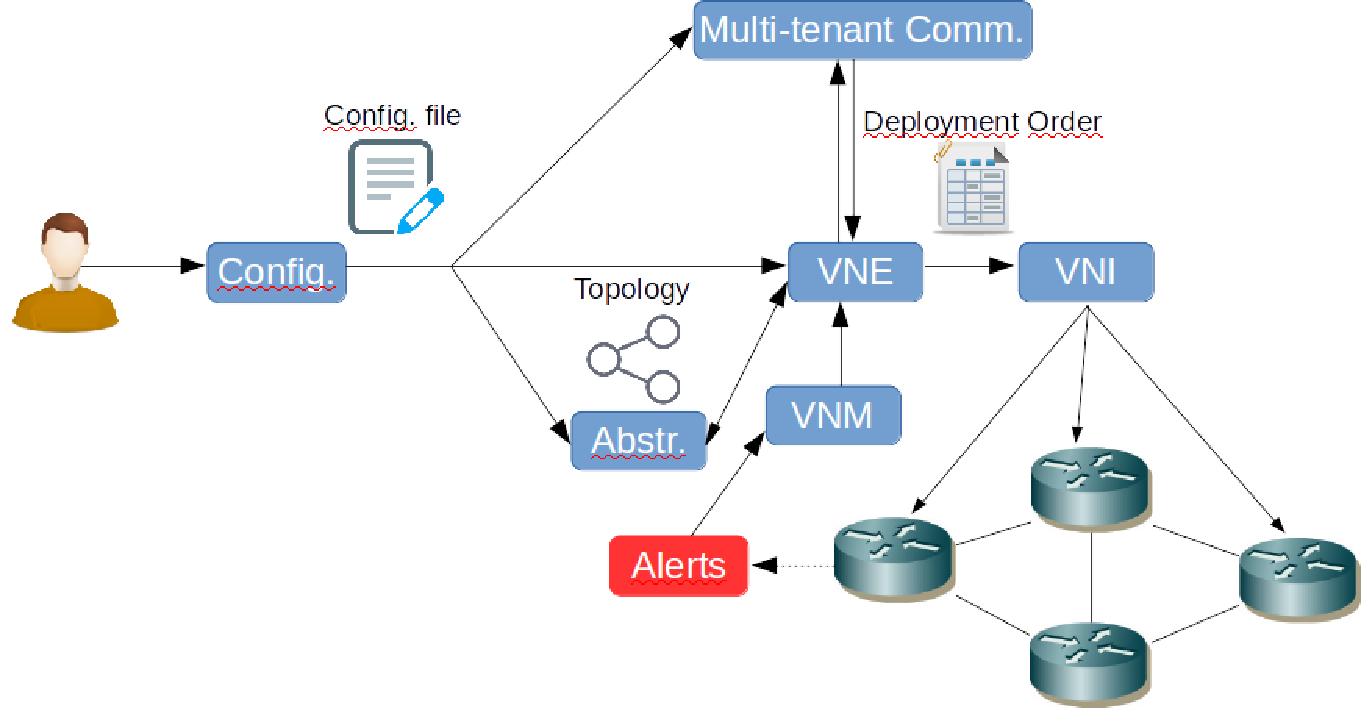
\includegraphics[scale=0.7]{figures/network-hypervisor-workflow}
% \caption{Deploying a topology in a network hypervisor.\label{fig:Workflow}}
% \end{figure}

% \subparagraph{\textbf{Migration}}\textbf{}\\
% The migration component collects alerts from the infrastructure about failures or resource congestion.
% Figure~\ref{fig:Workflow} illustrates how the component receives an infrastructure alert and transmits it to the VNE component so he can recompute the topologies.

% During runtime, a user may push a request for resources.
% This request is transmitted to the RAC for verification.
% If the request can be granted, the RAC will notify the VNI to deploy the resources.
% Oherwise, an error should be raised and returned to the user.





\subsubsection{Summary}
We have presented a reference based on existing network hypervisors using the SDN paradigm.
Table~\ref{tab:comparison-refarchi} summarizes it and shows how each hypervisor implements the different modules of the reference architecture.
Both DPAC and CPAC are implemented in every hypervisor, as they are essential for a basic support of network virtualization.
The control over the VN exposed by the CPAC is either hypervisor based (HB) or full control (FC).
% Openflow~\cite{Openflow-McKeown2008} is the main implementation for the DPAC as it is a standard supported by the industry and is widely studied.
Maintaining a mapping between physical and virtual resources in the DPAC has become a main goal since arbitrary topologies often come with flowspace virtualization, thus giving tenants a lot of flexibility.
Only Compositional Hypervisor~\cite{CompositionalHypervisor-Jin2014} does not properly virtualize the dataplane and interact with it using OpenFlow~\cite{Openflow-McKeown2008}.
In a similar way, the VNE algorithms greatly simplifies the administration of virtual networks and thus has been integrated since early prototypes.
While FlowVisor provides CPU and bandwidth (BW) isolation, only Slices Isolator~\cite{SlicesIsolator-El-Azzab2011} and Double FlowVisor~\cite{DoubleFV-Yin2013} extend this isolation to the interfaces (Int) of a switch as well as the memory (Mem).
We observe that few solutions have implemented an advanced monitoring module (\ie monitoring more than Discovery Protocols Notifications).
In addition to that, network hypervisors rarely address the migration problem, leaving a lot of work to do to researchers.




% Please add the following required packages to your document preamble:
% \usepackage{multirow}
% \usepackage{graphicx}
\begin{table}[]
\centering
\resizebox{\textwidth}{!}{%
\begin{tabular}{|c|c|c|c|c|c|l|}
\hline
Name                                                            & CPAC                      & DPAC          & Topology      & VNE & VNM & Security \\ \hline
FlowVisor~\cite{FlowVisor-Sherwood2009}                         & \multirow{6}{*}{FC} & Proxyfication & Not arbitrary & No  & No  & No       \\ \cline{1-1} \cline{3-7} 
ADVisor~\cite{ADVisor-Salvadori2012}                            &                           & Mapping       & Arbitrary     & No  & No  & No       \\ \cline{1-1} \cline{3-7} 
VeRTIGO~\cite{VeRTIGO-Corin2012a}                               &                           & Mapping       & Arbitrary     & Yes & Yes & No       \\ \cline{1-1} \cline{3-7} 
Enhanced FlowVisor~\cite{EnhancedFV-Min2012}                    &                           & Proxyfication & Not Arbitrary & No  & No  & No       \\ \cline{1-1} \cline{3-7} 
Slices Isolator~\cite{SlicesIsolator-El-Azzab2011}              &                           & Proxyfication & Not Arbitrary & No  & No  & No       \\ \cline{1-1} \cline{3-7} 
Double FV~\cite{DoubleFV-Yin2013}                               &                           & Mapping       & Arbitrary     & Yes & No  & No       \\ \hline
Compositional Hypervisor~\cite{CompositionalHypervisor-Jin2014} & FC                  & Openflow      & Not Arbitrary & Yes & No  & No       \\ \hline
CoVisor~\cite{CoVisor-Jin2015}                                  & FC                  & Mapping       & Arbitrary     & Yes & Yes & Yes      \\ \hline
FlowN~\cite{FlowN-Drutskoy2012}                                 & HB                       & Mapping       & Arbitrary     & Yes & Yes & No       \\ \hline
Network Hypervisor~\cite{NetworkHypervisor-Huang2013}           & HB                       & Mapping           & Arbitrary     & Yes & No  & No       \\ \hline
AutoSlice~\cite{AutoSlice-Bozakov2012,AutoSlice2-Bozakov2014}   & FC                  & Mapping       & Arbitrary     & Yes & Yes & No       \\ \hline
NVP~\cite{NVP-Koponen2014}                                      & FC                  & Mapping       & Full Mesh     & No  & Yes & Yes      \\ \hline
OpenVirteX~\cite{OpenVirteX-Al-Shabibi2014}                     & FC                  & Mapping       & Arbitrary     & Yes & No  & No       \\ \hline
SR-PVX~\cite{PVX-Li2017}                                        & FC                       & Mapping       & Arbitrary     & Yes & No  & No       \\ \hline
WhiteVisor~\cite{whitevisor-Yu2019}                             & FC                 & Mapping       & Arbitrary     & Yes & No  & No       \\ \hline
ONVisor~\cite{ONVisor-Han2018}                                  & HB                       & Mapping       & Arbitrary     & Yes & No  & Yes      \\ \hline
LiteVisor~\cite{Litevisor-Yang2018}                             & FC                  & Mapping       & Arbitrary     & Yes & Yes & No       \\ \hline
\end{tabular}%
}
\caption{Comparison of the network hypervisors with the reference architecture}
\label{tab:comparison-refarchi}
\end{table}

\newpage
\section{Migration of virtual networks with SDN}
\label{sec:sota-vnmigration}
In this section, we discuss the different virtual network migration solutions.


\subsection{Preliminary work}

We start by presenting solutions published on the same year as OpenFlow and that have been used as a reference in a majority of SDN-based migration solutions.

\subsubsection{VROOM}
Virtual ROuters On the Move (VROOM)~\cite{VROOM-Wang2008} is an early work discussing how the migration of virtual routers should be implemented on top of the physical infrastructure. 
VROOM outlines that most of the network state changes are caused by planned maintenance.
Moreover, power consumption is also a primary concern because efficient migrations can save up to hundreds of millions of dollars.
In this regard, VROOM presents a network virtualization and migration technique aiming at minimizing these costs and the duration of maintenance.
VROOM is composed of 3 building blocks: router virtualization, data and control plane separation, and dynamic interface binding.
Router virtualization is already implemented in some commercial routers, and VROOM presents two prototypes, one software based and the other one hardware based.
Data and control plane separation is achieved by using different virtualization environments (VE) in a virtualization infrastructure, namely OpenVZ~\cite{openvz}.
The data plane is implemented using OpenVZ first VE (VE0) in which the software implementation of the VROOM router will use a Linux kernel in a commodity server while the hardware implementation will use a NetFPGA circuit.
The control plane is also implemented using OpenVZ but using separate VEs (VE1, VE2, ...).
Each virtual router is stored in a VE, in which a kernel and routing protocol are implemented using a software suite.
The binding of physical interfaces with virtual interfaces is divided into two mappings.
The first one implements the mapping of the virtual router with the corresponding Forwarding Information Base (FIB) inside the physical router.
The second one is the mapping of the FIB of the physical router with a corresponding physical interface.

\subsubsection{Virtual Network Embedding and path migration}
Yu~\etal proposed in~\cite{VNE-Yu2008} a VNE model designed to support the splitting of a virtual link over several physical links, as well as dynamic virtual network reconfiguration.
The whole work is intended to improve resource allocation and maximize the acceptance rate. 
Path splitting takes a virtual link with a required amount of bandwidth that cannot be embedded on the physical infrastructure, and divides it into several smaller links that can be accepted by the infrastructure.
Several VNE algorithms are proposed, including one tailored to fit a type of topology that is expected to be common.
Path migration extends the usability of path splitting by allowing to recalculate the embedding of existing virtual networks and freeing extra resources otherwise not available using path splitting solely.
The authors provide an extensive evaluation of their mapping and migration algorithms using a simulator~\cite{vnesimulator}.

Both~\cite{VROOM-Wang2008} and~\cite{VNE-Yu2008} have been published on the same year as the publication of OpenFlow~\cite{Openflow-McKeown2008}, an implementation of the Software Defined Network paradigm that will become the standard of SDN for both industry and academia.
Despite the fact that these publications are not based on SDN, they set up guidelines for plenty of the works we will now describe.

We divide the existing VN migration solutions based on the research issue they tackle.
% \GB{the categorization seems to explore 3 different objectives, and it is difficult to see the logic of such categorization}
We summarize these issues into three categories: 
\begin{inparaenum}[i)] 
\item the migration is designed to improve the global performance of the infrastructure;
\item the migration was implemented to explore existing technical limitations with regard to virtualization platform; or 
\item the solution explores the migration from a formal perspective.
\end{inparaenum}

\subsection{Improving the performance of the infrastructure}
% Ye~\etal propose in~\cite{Ye2017a} a resource utilization model in which they aim to maximize the resource allocation on switches while looking to determine controllers that can be shut down due to underutilization and migrate switches.
% Authors solve the resource allocation problem using optimization under constraints techniques. 
% The switch migration problem is described as NP-hard and is approximated using a Log-sum-exp approximation.
% This approximation determines the allocation of network switches on controllers that will maximize their utilization. 
% From this distribution, authors construct a Markov chain that represent the different distributions strategies and where transitioning from a state to another corresponds to migrating a switch from a controller to another controller.

% In~\cite{Wang2017d}, Wang \etal study a problem similar to~\cite{Ye2017a}, but are more focused on the migration and its efficiency, and present a Switch Migration-based Decision Making (SMDM) scheme. The problem is divided into three parts: detecting the overload of the controller due to an excessive amount of OF requests, the modeling of the migration's performance and finally, modeling the trade-off between the profit generated by the migration and the cost it incurred.
% The overload detection correlates two types of information to determine overloaded controllers.
% The first one is the actual amount of requests received by controllers, while the second is the load ratio between each pair of controllers.
% This ratio is then bound to a threshold above which a migration will be triggered to relieve one controller from its load and reallocate it to the other.
% Modeling the efficiency of the migration considers both the load variation of the controllers as well as the overhead of messages exchanged to implement the migration.  
% Finally, the migration strategy is in charge of determining which switch should be selected as the next candidate for the migration and where it should be migrated.
% Figure~\ref{fig:smdm-wang2017d} illustrate the interactions of the different components of the solution.

% \begin{figure}[ht]
%     \centering
%     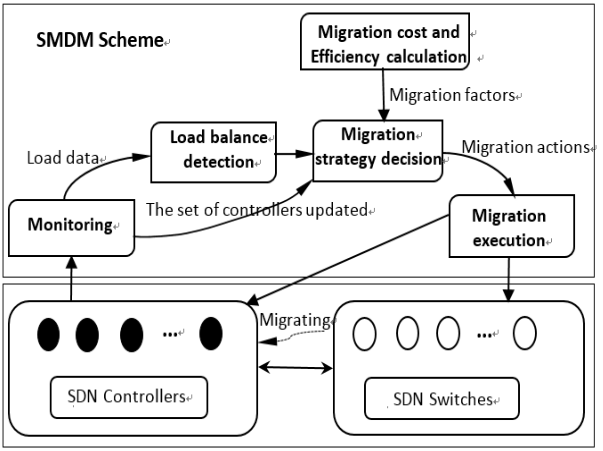
\includegraphics[scale=0.65]{figures/wang2017d.png}
%     \caption{Architecture of the SMDM scheme~\cite{Wang2017d}}
%     \label{fig:smdm-wang2017d}
% \end{figure}

Lo~\etal introduce in~\cite{vnm-lo2013} the design of a virtual network migration process.
The cost of the migration is based on two metrics, the completion time of the migration as well as the bandwidth consumption.
Based on the original embedding and the new destination substrate, the goal is to determine the ordering of node migration that will minimize the cost of the migration.
For each step in the migration, the time taken to migrate a node is divided into two parts. The first one represents the time taken to prepare the migration and the second one is the time taken to actually transmit information to the destination substrate.
The cost of a migration step is the product of the time it takes to migrate the information with the impact the migration incurs on the bandwidth.
Virtual nodes are categorized based on whether the node:
\begin{inparaenum}[i)] 
\item has been migrated;
\item will be at this step of the migration; or 
\item will be migrater at a later step.
\end{inparaenum}
Similarly, the virtual links' are divided into three categories based on whether the nodes composing the links:
\begin{inparaenum}
\item have been migrated;
\item will be migrated; or 
\item will not be migrated.
\end{inparaenum}
The categorization of virtual resources is then used to determine the cost of the migration.
Three different virtual network migration algorithms are presented, differentiated by the fact that nodes may be either migrated one node at a time or multiple nodes may be migrated together.
% \GB{three algorithms but only 2 are mentioned. and don't you ever use ``whether'' again?}
The first algorithm is a greedy iteration over the individual costs of migrating each node.
The second algorithm is designed to minimize the migration time. Since migrated nodes are constrained to be independent from other nodes, the algorithm determines the biggest set of independent nodes.
Then, the algorithm leverages the fact that several nodes can be migrated simultaneously to reduce the total migration time.
The third algorithm is a combination of the first two, where a tradeoff between migration time and migration cost is sought. The algorithm computes the different sets of independent nodes, and instead of choosing the largest one, choose the set with the smallest cost.
Again, this algorithm uses the simultaneous node migration to choose the set with the smallest cost.

Robust virtual network migration is studied in~\cite{Ko2017c}. The authors outline that traditional migration suffers from down times proportional to the size of the migrated virtual networks, while protection mechanisms cannot be adapted to support the dynamic changes in the network.
Three requirements are defined while considering drawbacks of existing migration techniques. 
First, the tenant's controller should never be notified of the migration.
Second, the migration process should account for the network traffic status inside the physical infrastructure.
Finally, the migration process should minimize the number of interactions between the network hypervisor and the physical infrastructure.
Protection and restoration techniques are described to account for these requirements.
Protection consists in deploying backup paths on the physical nodes, calculated prior to any incident.
This way, in case of a failure, the traffic can immediately be routed through the alternative path. 
This method implies that the hypervisor must maintain regularly updated backup paths in each node, incurring computational overhead, bandwidth consumption on the physical resources of the switch.
Restoration is the case where all the backup paths are stored inside the network hypervisor and only deployed in case of a failure.
This method is based on the assumption that failures will rarely happen, thus it will not generate an important number of messages between the infrastructure and the hypervisor.
The network hypervisor determines a backup path that will minimize the amount of messages sent to the infrastructure.
To do so, the backup path must use the same links as the original while only differing at the failure point.
Updates of backup paths are performed regularly while a monitoring device collects statistic on available resources to determine if the current backup paths can still be used.
The migration solution is implemented using OpenVirteX~\cite{OpenVirteX-Al-Shabibi2014}, where the path calculator and storage mechanisms are adapted to fit the new requirements. 
% Then new components related to the prioritization of backup paths, updating existing paths and monitoring the physical network are implemented and integrated into the hypervisor.

Improving the revenue generated with network virtualization can be done through migration.
In~\cite{fragment-Liu2018}, the purpose of VN migration is to optimize the acceptance ratio of new virtual network requests as well as the revenue to cost ratio.
While traditional VNE algorithms only rely on the individual capacities of nodes, they do not consider the possibility to split the bandwidth over multiple links.
To this end, the notion of fragment degree for a virtual node is introduced and is defined as a weighted combination of the CPU consumption ratio of the virtual node on its embedding node and the bandwidth consumption ratio of adjacent virtual links on the physical substrate.
The fragment degree of each virtual node is then associated with the embedding cost of existing virtual networks into a multi-objective integer linear program. The solution of this program being NP-hard to solve, the authors propose a novel algorithm to make it computationally tractable: Fragment-aware Virtual network Reconfiguration (FA-VNR).
This algorithm first defines a migration trigger. 
% Maximizing revenue over time pushed for a periodical migration of VNs.
Then, it determines which set of physical nodes must be reconfigured by computing a dynamic threshold of ``fragmentation" in the infrastructure.
Similarly, the algorithm determines a set of virtual nodes to migrate based on their economical performance.
Once the destination substrate has been chosen, virtual nodes will be migrated and each virtual link connected to them will be redeployed using a shortest path algorithm.

\subsection{Evaluating virtualization platforms}
We present here two migration solutions that have been implemented on a particular physical infrastructure.
Both solutions aim at outlining the technical limitations faced when migrating VNs.

\subsubsection{PlanetLab}
PlanetLab~\cite{Chun2003d} (PL) is a virtualization infrastructure used to provide slices of network resources for research experiments. Lo~\etal state in~\cite{Lo2014} that VN migration is a field where practical implementation and evaluation remain to be explored. They proposed a migration scheme and implemented it in PL, namely PL-VNM. The migration should be designed to be automated, fast and to minimize the service disruption time. While the migration process is automated, there is no detection component to automatically trigger the migration. Due to technical limitations of PL, it is impossible to migrate a VN from a slice to another. An alternative is proposed by partitioning the resources within a slice thus defining new virtual networks inside a PL slice and limiting the migration to the VNs created in a single slice. Virtual routers are instantiated for each virtual node required by the topology, and use an API to install forwarding rules in the kernel space of the physical node.
The authors proprose a simple migration algorithm based on the size of the flows to migrate.
The migration process consists in cloning the network state of virtual nodes (\ie FIB) and then  redirect VMs' traffic through the newly created virtual network.
While the duplication of networking state does not cause any packet loss from the tenant's point of view, setting up the redirection is most likely to create service disruption.
Two different approaches are taken and evaluated.\\
The first approach consists in preparing the scheduling for the host redirection and then sequentially send commands to the gateways connected to the hosts, namely remote scheduling.
Figure~\ref{fig:plvnm} depicts the modules of PL-VNM and how the migration process is handled.
One of the drawbacks of this method is the delay existing between the migration instruction being sent by the controller and the instruction actually being run at the gateway.\\
The second approach relies on determining the migration ordering and then scheduling the migration in the gateway using the UNIX command \textit{at}. The \textit{at} command makes sure that the migration is performed on time by synchronizing the gateway via the NTP protocol. Here, the potential latency to execute the migration is based on the time it takes for NTP to trigger \textit{at} and on the load of the gateways' CPU.
Both approaches make it hard to have a full control over the migration's timing.
The authors conclude with three recommendations for the PL infrastructure and in general for network hypervisors.
\begin{inparaenum}[i)]
\item Enabling gateway task scheduling with a magnitude order of milliseconds. As is, \textit{at} scheduling uses seconds for tasks triggers while path latency of remote scheduling is a few hundreds of ms;
\item Allowing the migration scheduler to order migration commands to reduce the delay induced in the actual start of the command;
% \GB{to be rewritten}
\item Implementing asymmetric packet routing inside the infrastructure.
Because of the routing mode used in PL, each link in the gateway must have the same physical source and destination, thus preventing an asymmetric migration of the FIB from being effective. 
\end{inparaenum}

While~\cite{Lo2014} is not specifically designed to work on an SDN infrastructure, the problems and challenges it explores remain valid in the SDN paradigm.

\begin{figure}[ht]
    \centering
    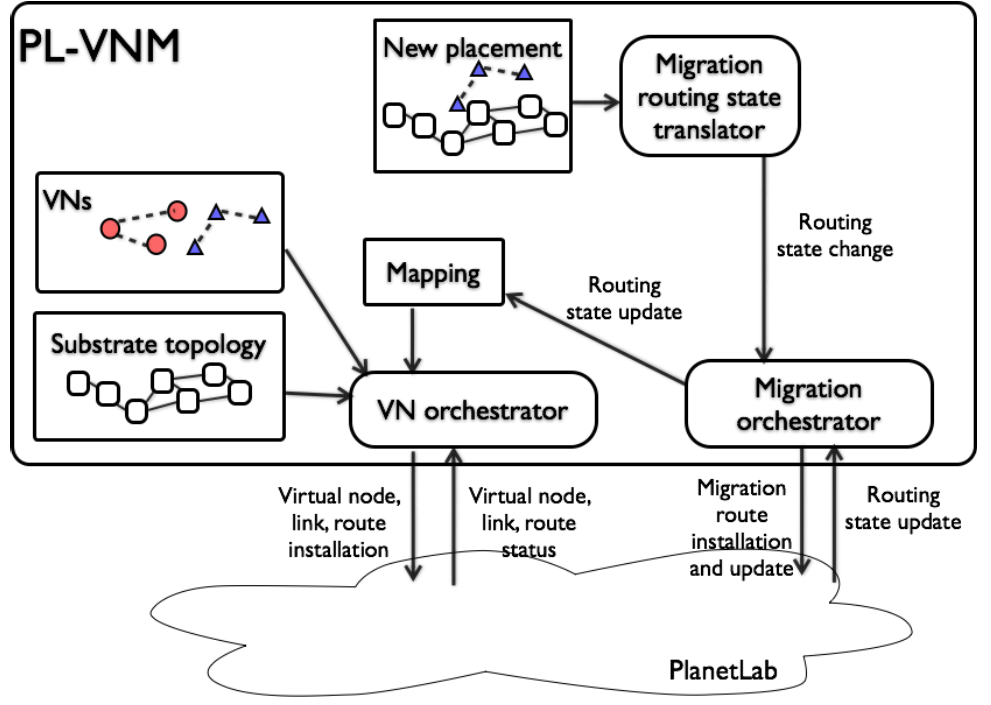
\includegraphics[scale=0.5]{figures/pl-vnm.png}
    \caption{Architecture of PL-VNM~\cite{Lo2014}}
    \label{fig:plvnm}
\end{figure}

\subsubsection{GENI}
The GENI platform~\cite{GENI-Berman2014} is a network infrastructure based on SDN and used to provide isolated environments for researchers to run experiments.
Zhao~\etal propose in~\cite{Zhao2017} a VN migration scheme implemented using GENI. 
Similarly to PlanetLab, GENI has not been designed to support the migration of VNs over different physical substrates. 
We differentiate \textbf{slice} from \textbf{Virtual Networks (VN)} in~\cite{Zhao2017}.
A \textbf{slice} is a GENI slice, \ie the set of resources allocated to a tenant, while \textbf{VN}  are a subset of these resources.
Implementing VNs (original and migration backups) can be done by allocating all required resources to a single slice. This approach comes with drawbacks however: no clear isolation between VNs, lack of flexibility in case there is a need for a topology change. Finally, in case of a failure of a VN or a host, the whole topology must be rebuilt.
Another approach consists in allocating one slice for a single VN and then, when migrating it, allocating a new slice. The main challenge is to set up communication between the old and the new slice during the migration, since GENI enforces isolation between its slices.
In addition to the inter-slice communication, the migration process should not cause packet loss and be invisible to the tenant.
A proposed approach separates the old VN, the new VN and the VMs by setting up a different slice for each group. Two extra gateways are inserted in the VMs' slice, each connected to one of the other slices.
Without these gateways, the learning switch implemented by GENI would not allow to connect the hosts to the new VN because of conflicting rules (same source/destination, different output ports).
The three slices will then share a common VLAN to communicate together.
In order to minimize the packet loss incurred by the migration, the migration is optimized by scheduling the sequence of flows that will be deployed on the physical substrate.
First the rules between gateways and the new VN are set up, then the hosts' traffic is redirected towards the second gateway and finally old VN rules are dropped leading to a full disconnection of the former VN.
A similar problem to the migration in PlanetLab concerns the migration scheduling on the physical switches.
The first option is to remotely control network interfaces using SSH.
An SSH connection with each switch is established and old interfaces will be shut down while activating the new ones.
However, the latency induced by SSH authentication and by the time it takes to transmit commands makes the migration unpredictable.
On the other hand, the migration can be performed by sending OF rules as the migration progresses. This method is deemed faster than the other one since it does not use SSH (and its authentication overhead), but it is thus less secure.
Finally, the transparency of the migration is ensured by the migration controller who will act as a proxy between VNs and switches, intercepting packets and rewriting header fields to maintain a consistent view of the network.

\subsection{Formal verification of the migration}
In complement to the works aiming at improving the performance and the scalability of the virtualization infrastructure and the migration process, we now consider the works taking a formal approach to study specific properties of the migration and the migration process. 
% \GB{ok but to what ends?}
The following approaches contrast with the previous ones because they characterize specific properties of the migration of virtual networks instead of focusing on operational aspects. 

\subsubsection{Inter-flow consistency}
In an SDN infrastructure, the configuration deployed on SDN switches gets updated and evolves regularly. Such modifications are invoked by the SDN controller and deployed among several switches.
Flow consistency ensures that each flow will be processed by either the old or the new configuration all along the way, and not by a combination of the two.
However, Liu~\etal argue in~\cite{Liu2015a} that making sure that each individual flow has its own consistency preserved is not enough to respect certain security and reliability requirements.
It becomes necessary to model relationships between flows and to preserve certain properties throughout the migration.
The properties considered here are spatial isolation and version isolation.
The spatial isolation of two flows consists in preventing them from sharing a common physical resource before, during and after a change in the network configuration.
For instance, a critical flow carrying important information should not share a link with a certain traffic that may be subject to surges, thus leading to link congestion and the important flow not being delivered. Another case would be when attackers would try to intercept information on critical flows and then exploit the infrastructure.
Version isolation ensures that a configuration affecting different flows is fully deployed and prevents one flow being processed with one configuration and another flow with another version of the configuration.
This problem is related to the delay in actually deploying the configuration inside the switches, as outlined with PlanetLab and GENI.
The spatial isolation problem is approached using a dependency graph. Each path taken by a flow is mapped with the physical nodes they go through. Then, in case of overlapping node for several flows, the node is seen as a mutex node (similarly to the mutex of an operating system).
No flow may go through a mutex node if another flow is currently using it.
This ensures that specific traffic may not cohabit inside the same physical resources.
To ensure the version isolation of different flows, the system identifies the set of flows that must be isolated. Then, it picks one to be processed normally and forward to the controller all the traffic of the remaining flows. This way, it makes sure that there are not two flows being processed by 2 different versions of a configuration. And when all the cached traffic is re-injected inside the infrastructure, it is being processed by a fully updated networking state.

The generation of the dependency graphs is done by categorizing flows into two classes, based on whether they should be forwarded to the hypervisor or not. Using a greedy algorithm, we can determine how to minimize the amount of packet caching that would be done at the controller.
The ordering of the migration sequences is determined from the graph. Each sequence is composed of several configuration modifications, and these modifications are also ordered to minimize the migration time. 

\subsubsection{Moving Target Defense}
Dynamically changing the location of sensitive targets is a technique called Moving Target Defense (MTD). Such changes prevent an attacker from accurately knowing the attack surface of the system he is attacking. 
% because the configuration regularly changes. 
% \GB{all the segment on the works of Chowdhary does not really concern migration. you may drop it}
Chowdhary~\etal~\cite{Chowdhary2016} use MTD techniques as part of a Detect-Analyze-Counter cycle inside an SDN-based Cloud infrastructure. 
The security system is composed of four modules: a detection module, a vulnerability analyzer, a counter-measure creation and deployment component and a policy conflict resolution.
The detection module is in charge of gathering information about the vulnerabilities in the infrastructure.
Then, the analyzer will use these information to dynamically generate an attack graph representing the capacities of the attacker. 
A counter-measure will then be generated to mitigate the potential attacks and be proposed to the conflict resolution module. This module  will determine if the newly created counter-measure is not going to have any harmful side effects. Once the counter-measure is accepted it is deployed in the infrastructure and the detection module is notified of the new configuration. 
The attack detection aspect is left out in this paper, as it is already a widely explored topic.
A well known drawback of attack graphs is the poor scalability when the number of states grows.
This problem makes the graph generation computationally intractable. Partitioning the attack graph into smaller regions based on each tenant using the infrastructure simplifies the generation.
These sub-attack graphs are then simply merged together for the counter-measure to be generated.
The counter-measure component determines which VM should be migrated based on the CVSS Base Score.
Once the target VM is chosen, new flow rules are computed to implement the migration. 
The conflict resolution inspects the flow rules that should be deployed and extracts the actions of each rule and verify that they do not overlap with other existing flow rules. If a conflict arises, this module will try to find alternative rules. In the event where this would not be possible, the proposed counter-measure is rejected and a new one is computed.

\subsubsection{Seamless migration}
In the previous works, minimizing the service disruption caused by the migration has always been a major concern in the design of the solution. However, while the efficiency of the solution was evaluated with various experiments, there was no formal approach describing the transparency of the migration and ensuring that no disruption of service will be experienced by a tenant.
The topic of seamless migration is brought up in~\cite{toward-Ghorbani2014} where Ghorbani~\etal take a closer look at network virtualization using SDN techniques.
Precisely, the focus is put on the one-to-many mapping, also known as the ``Big Switch" abstraction.
Distributing a single virtual resource over several physical ones may not preserve the per-flow correctness.
Similarly to the version isolation presented in~\cite{Liu2015a}, flow correctness considers flows individually and ensures that each packet of each flow  is always processed by one specific version of a network configuration. 
% Version isolation ensures that flows are processed by a single global configuration while flow correctness ensures that end points receive packets in the proper order to avoid errors at the application level.
However, this definition does not ensure that the ordering of packets as seen by the tenant's applications and controllers is a good representation of how the packets were originally sent and ordered by the other end point.
A new definition of correctness is proposed to make sure that the ordering of packets is preserved from end to end.
From this definition  a solution for a seamless migration of VNs and VMs is proposed in LIME~\cite{Lime-Ghorbani2014}.
The first contribution of this paper is a formal model for network virtualization migration, and it defines a transparency property related to the physical observation of the migration.
The second is an implementation of a virtual network migration process that is proven to respect the transparency property previously defined.
It is important to note that transparency does not exclude packet loss but is aimed to reduce it drastically.
The migration of the virtual network resources relies on switch cloning.
LIME will instantiate several copies of each virtual node and orchestrate the migration so the tenant's traffic is still forwarded during the migration.
In opposition to the requirement made in~\cite{Ko2017c}, LIME will notify the tenant application in case of a physical failure of a link.
Ghorbani~\etal then use the formal model to extend the transparency property to the one-to-many mapping problem of~\cite{toward-Ghorbani2014}.
Since the idea is to propose a ``Big Switch" abstraction while  the virtual resource is being replicated across several physical nodes. The point is to make sure that all nodes located on the edge of the Big Switch are preserving the ordering of the packets even when the configuration is updated.
The observation correctness introduced in LIME is enhanced with the concept of weak causality where an event has weak causal dependency with another if the first event has triggered the other under certain conditions.
Thus, the observable ordering of events will matter only if those events are correlated.


\subsection{Summary}
The study of VN migration remains a topic of interest as it has been studied but often with the same objective: creating a migration process that will improve the performance of the infrastructure. 
Table~\ref{tab:existing-vnm} summarizes the surveyed works. Several types of algorithms are proposed, usually either a migration scheduling algorithm or a VNE-related algorithm. 
The bandwidth remain the most common metric used, as it is one of the main criteria to support virtual networks. Other operational metrics like migration duration or CPU consumption are used for performance improvement.
The migration process has not been studied under the security perspective.
This should be investigated to propose a model of the security of the migration process, its properties and how can they be observed and verified. From an architectural point of view, users are not presented with their own virtual network that they will be able to configure, but instead the manipulation of the physical infrastructure is abstracted to implement an efficient OF rules deployment and to allow the coexistence of heterogeneous solutions.

% Please add the following required packages to your document preamble:
% \usepackage{graphicx}
% \GB{please insert authors' names in the reference column of Table~\ref{tab:existing-vnm}}
\begin{table}[h]
\centering
\resizebox{\textwidth}{!}{%
\begin{tabular}{|l|l|l|l|}
\hline
\textbf{Reference}       & \textbf{Algorithms}                                                                                                          & \textbf{Metrics}                                                                              & \textbf{Summary}                                         \\ \hline
Wang~-~\cite{VROOM-Wang2008}    & N/A                                                                                                                          & \begin{tabular}[c]{@{}l@{}}Power consumption\\ Bandwidth\\ CPU\end{tabular}                   & Early prototyping virtual network migration              \\ \hline
Yu~-~\cite{VNE-Yu2008}        & \begin{tabular}[c]{@{}l@{}}Link/Node mapping\\ Path splitting\\ Path migration\\ Custom topology mapping\end{tabular}        & \begin{tabular}[c]{@{}l@{}}CPU\\ Bandwidth\\ Request processing time\end{tabular}             & Migration to improve the acceptance ratio                \\ \hline
Lo~-~\cite{vnm-lo2013}        & \begin{tabular}[c]{@{}l@{}}Greedy minimum cost\\ Biggest set of independent nodes\\ Biggest set  + minimum cost\end{tabular} & \begin{tabular}[c]{@{}l@{}}Migration duration\\ Bandwidth\end{tabular}                        & Scheduling algorithms for the migration                  \\ \hline
Ko~-~\cite{Ko2017c}           & Backup path computation                                                                                                      & Bandwidth                                                                                     & Migration module on top of OpenVirteX                    \\ \hline
Liu~-~\cite{fragment-Liu2018}      & \begin{tabular}[c]{@{}l@{}}Target selection\\ VNE\end{tabular}                                                               & \begin{tabular}[c]{@{}l@{}}CPU\\ Bandwidth\end{tabular}                                       & Improving the acceptance ratio                           \\ \hline
Lo~-~\cite{Lo2014}            & Flow size based migration                                                                                                    & \begin{tabular}[c]{@{}l@{}}Packet loss\\ Migration time\end{tabular}                          & Implementing VN migration on PlanetLab~\cite{planetlab}  \\ \hline
Zhao~-~\cite{Zhao2017}          & Seamless traffic redirection                                                                                                 & \begin{tabular}[c]{@{}l@{}}Packet loss\\ Migration time\\ Control plane overhead\end{tabular} & Implementing VN migration on GENI~\cite{GENI-Berman2014} \\ \hline
Liu~-~\cite{Liu2015a}          & \begin{tabular}[c]{@{}l@{}}Flow classification\\ Mutex nodes\\ Migration scheduling\end{tabular}                             & \begin{tabular}[c]{@{}l@{}}Bandwidth\\ Memory\end{tabular}                                    & Consistent flow processing during configuration changes  \\ \hline
Chowdhary~-~\cite{Chowdhary2016}     & \begin{tabular}[c]{@{}l@{}}Attack graph analysis\\ Counter measure selection\end{tabular}                                    & Vulnerabilities                                                                               & VN migration for VM security                             \\ \hline
Ghorbani~-~\cite{Lime-Ghorbani2014} & \begin{tabular}[c]{@{}l@{}}Node cloning\\ Iterative migration\\ Simulataneous migration\end{tabular}                         & \begin{tabular}[c]{@{}l@{}}Latency\\ Packe loss\\ Bandwidth\\ Network updates\end{tabular}    & Formal verification of the seamless migration            \\ \hline
\end{tabular}%
}
\caption{Summary of VN migration}
\label{tab:existing-vnm}
\end{table}


\subsection{Security of VM migration}

In this section we take a closer look at the security of the live migration of VMs.
We first detail the existing vulnerabilities and attacks possible and then detail different security solutions, either using the migration process as a way to overcome security issues or that analyze and improve the security of the migration process itself.

\subsubsection{Attacking the VM migration process}
Traditional hypervisors have been around for decades now, and the live migration of a virtual machine is a well known process. There has been several security surveys on the topic of VM hypervisors~\cite{Reuben2007,Rehman2013,Sahoo2010,Perez-Botero2013}, and on the security of Cloud environments~\cite{cloudenvironmentsecuritysurvey-fernandes2014}.
Most of the security issues with VMs are related to the unlawful interactions between a VM and other VMs or the hypervisor.
An attacker may exploit vulnerabilities in the hypervisor and force it to execute arbitrary code or access restricted memory zone.
Another type of attack consists in corrupting the resource scheduler of the hypervisor, thus preventing other users to get the allocated resources they deserve.
We will focus here on the attacks that can impact the (live) migration of a VM.
Oberheide~\etal proposed in~\cite{empirical-oberheide2008} several attack classes that will affect the migration of VMs: attacks on the control plane, the data plane and the migration module.
First of all, attacks impacting the control plane can be summarized into two categories. The attacker is triggering unlawful migration either to move a VM toward an unsecured physical location or to overload the local hypervisor and preventing a legitimate user to be served with his due resources.
The second attack consists in Fake Resource Advertising. This kind of attacks are particularly efficient in systems where the migration is automated, because the generation of fake servers inside the topology can make the hypervisor trigger migration of VM on resources that do not exist.
Attacking the data plane during the live migration can take two forms: passively exfiltrating sensitive information or actively altering the traffic during the migration.
In the first case, the attack result in a loss of confidentiality for the stolen data and it might be exploited later on to launch other attacks on the VM.
In the second case, altering the traffic can either create a Denial-of-Service because the VM virtual disk has been compromised, or in a potentially even more harmful scenario the VM keeps working but under a compromised state, as the ongoing processes may not function with expected data.
The VM migration process can also be attacked to allow an attacker to have his VM share the same physical server with his victim's VM. Stalling the migration is studied in~\cite{stalling-atya2017} where the attacker prevents his and his victim's VMs from being separated so he can completely invalidate the memory pages of the victim's VM. It is shown that maintaining the co-residency between the VMs allows an attacker to use side channels attacks that will have a bigger impact on the victim.
A presentation on these side channel attacks is shown in~\cite{malicious-atya2017}.

\subsubsection{Protecting the VM migration process}
The Moving Target Defense (MTD) paradigm is a common technique to limit the co-residency rate between an attacker and its victim, thus leading to a reduced attack surface for side channel attacks.
Zhang~\etal introduce a Game Theory model~\cite{incentivemtd-Zhang2012} to represent the incentives a Cloud Provider has to migrate VMs in his infrastructure versus an attacker who will benefit from the co-residency. Results show that it is not necessary to permanently migrate all VMs and only a subset of them. In addition to this, the game can be extended to include cooperation between the legitimate users and the Cloud Provider.
A similar approach using MTD against side channel attacks is presented with Nomad~\cite{nomad-Moon2015b}. Nomad is built on the assumptions that the attacker cannot be precisely located inside the infrastructure, can launch potentially unknown side channels attacks and can precisely target his victim. 
The migration process proposed in Nomad provides tenants with an API to describe a set of constraints on their VM that has to be respected throughout the migration.
Nomad provides a scalable VM placement algorithm, a framework that does not require to modify the OS, the hardware or the hypervisor, other than the migration algorithms.
Protecting the migration process by making undetectable by an attacker is studied in~\cite{stealth-Achleitner2017a}. Even if encryption is applied to the migration traffic, an attacker located inside infrastructure still may distinguish migration traffic from the legitimate one. Indeed, migration traffic can easily be characterized by as set of data bursts through the network. The solution proposed uses a token bucket traffic generator to implement a white noise that will dynamically adapt to the traffic generated by the migration. This method will make each traffic look like a constant flow of indistinguishable data.

\subsubsection{Summary}
We have presented a broad overview of the Live VM migration process.
Legacy hypervisors have extensively studied, and the use of the migration process has been used not only for maintenance purposes but to tackle security issues existing in virtualization infrastructure.
The security of the migration process has also been studied and outlined vulnerabilities existing in hypervisors.
We note that the migration process extends the attack surface of the hypervisor because it also relies on the network infrastructure to support the operations of the VM migration.
Additionally, the migration of VM across SDN networks has obtained some focus~\cite{Datacenters2014,Lin2013,Ibn-Khedher2015} and a security study should be considered as well.


\subsection{Formal Models for network security}

Formal models for network security cover a broad range of topics and applications.
We consider here the models providing a form of algebra to represent, to a certain extent different security properties. We categorized these models into three different sections: languages used for the security analysis of a communication protocol, languages used to implement a form of access control for an information system and finally languages used to describe the infrastructure enforcing the security services.

\subsubsection{Communication protocol analysis}
In computer networks, confidentiality and authentication of the communications were among the most important properties to measure and protect.
In~\cite{CSP-Schneider1996}, messages exchanged between users are described and characterized by a set of security properties.
The author uses the Communicating Sequential Processes (CSP) algebra to represent the different actors involved in a network communication, including a potential attacker. 
Considering the formalism of CSP, the system will be described with the events it can perform and by the traces it generates (\ie the different sequences of events realized by the system).
In a communication system, messages can be sent and received by users.
Therefore, the definition of the confidentiality of a message is maintained if this message was only received by his intended recipient and no one else.
CSP has been proven effective for the analysis of communication protocol where the messages exchanged between different users generate a trace of network events, while each message can be ciphered using encryption keys etc.

The security analysis of communication protocols heavily relies on the expressiveness of the language used to describe it and how the attacker's capacities are defined. HLPSL~\cite{HLPSL-Chevalier2004} is a protocol specification language used to model the temporal interactions between users in a communication network. Using temporal logic, HLPSL describes the interactions between users not in terms of messages exchanged to achieve the communication but rather describes the role(s) of each user. Such roles may then be combined into composite roles when a protocol involves sub-protocols.
The definition of a role is a set of variables, either shared between roles or only known to one role.
Then, each role includes a set of states, and the conditions that must be met to transition from one state to another. Transition conditions include messages to be sent or received or if a specific information has been received using a particular ciphering key.
HLPSL proposes a modular definition of an attacker, where his capacities would not be identical over the whole system.
This is true in current networks, where the heterogeneity of the infrastructure may expose different vulnerabilities.
Security properties are defined as logical predicates combined with temporal operators such as: always, sometimes in the past etc.
The evaluation of a protocol's security is performed using the AVISPA tool~\cite{avispa}, in which model checking techniques are used to determine the potential vulnerabilities existing in the protocol.

\subsubsection{Access Control based languages}
A common way to describe networking system is by representing the interactions between the users with Access Control Lists (ACL).
ACLs can be seen as a set of rules that will either allow or deny the right to perform a specific action, to let a specific flow go through a firewall etc.
Representing authorization depends on the level of abstraction desired.
For instance, Matousek~\etal proposed in~\cite{Matousek2008} an ACL model at the network level, where router configurations are converted into ACLs which then are represented using a specific data structure to provide conjunction/disjunction capacities to the model (\ie combining several configurations together).
The main contribution of the paper is to provide an automated analysis of the network state while considering the changes in the topology (\ie link failure) as well as the security rules in place.
The analysis determines if a specific flow (named property) will be let through the system considering the configuration in place. They illustrate this with the example of a web traffic flow from an host to a Web server, and determine that in case of a link failure this flow will not go through anymore because of existing filtering rules.

MulVal~\cite{mulval-Ou2013} extends the notion of ACL analysis by implementing attacks on the system. 
First of all, the model uses the Common Vulnerabilities and Exposures (CVE) to describe the vulnerabilities in the infrastructure. This approach is different from~\cite{Matousek2008} because CVE impacts workstations, services and (mis)configuration. The security aspect is no longer only limited to  Layer 3\&4 filtering.
With the use of CVE comes the definition of attacks on the system and how they are performed.
Instead of converting each CVE into a specific attack, MulVal leverages the language definition to define broader attacks.
Therefore, each time a vulnerability is discovered, it will most likely fall under an attack already existing, thus minimizing configuration time about the attack.
MulVal's reasoning system is implemented to take into account sequential combinations of events.
Indeed, an attack may not be a single access to a resource but instead an access to a resource, followed by a privilege escalation that is concluded by the execution or arbitrary code on a machine.
They illustrate this by implementing an attack on a webserver and using the rights of the webserver to access a fileserver and install a corrupted binary that will be later on executed by an innocent user.

Taking an extra step back in the abstraction level, OrBAC~\cite{orbac} describes Access Control policies at the organization level. Simply put, an organisation is an entity, in which a role (\ie group of users) will be given a permission to do a specific activity (\ie action) on a view (\ie object) in a certain context (\ie under certain conditions).
Security policies include permission, prohibition or obligation to perform an activity.
OrBAC also uses the notion of contexts~\cite{context-orbac} which represents the conditions that must be met to authorize (or prevent) a user to perform a specific task.
The OrBAC model defines security policies using a set of logical predicates. These predicates will then be used to represent the permissions granted to the user.
We consider here the work done in~\cite{Cuppens} to convert high level policies into practical firewall configurations. Thanks to the possibility to precisely distribute permissions to the users, it is possible to use OrBac in a ``white list" mode, even though firewalls may be configured with prohibitions (\ie dropping packets by default as the last rule.
Finally, OrBAC offers a conflict resolution module in charge of detecting conflicts between high level policies and may propose solutions to solve them.

\subsubsection{Infrastructure based languages}
In the previous sections we looked at formal models in general systems, and the details of the underlying infrastructure were not always either clear or even studied. We now consider solutions that have a closer link with the infrastructure used to support the specifications made with the language.

M2D2~\cite{M2D2-Morin2002} is a specification language used to correlate alerts raised by Intrusion Detection Systems (IDS) inside an Information System (IS).
M2D2 describes four types of information required to do the correlation: characteristics about the IS, vulnerabilities, security tools and events occurring in the IS.
The IS is characterized by its topology (connections between network equipments and hosts), and by the products installed inside hosts (\eg OS, software etc.)
The definition of a vulnerability in M2D2 corresponds to a specific configuration on a host.
That is, the configuration of a host is the set of the different products installed.
If a subset of this configuration corresponds to a vulnerable configuration described in CVE, then the host is vulnerable to this specific vulnerability.
The security tools are IDS located either on a host or in the network (HIDS and NIDS) and are used to generate events based on their capacity to detect vulnerabilities.
They are given a detection range, which means one specific IDS may not detect certain vulnerabilities or attacks because they do not fall under his scope of scrutiny (\eg activated signature on a misuse IDS).
Events generated by IDSs are either scans, when a vulnerability is discovered, or an alert when an attacker is currently trying to exploit a vulnerability.
M2D2 contributes to alert aggregation on three different aspects: single host aggregation, target identification and false positives detection.
Single host aggregation regroups the alerts generated by the HIDS and the alerts generated by NIDS targeting this host.
Identifying targets vulnerable to a specific ongoing attack works by extracting the vulnerability exploited from the alert, then retrieving the associated configuration and determining if this vulnerable configuration is a subset in the configuration of each host in the IS.
Detecting false positives generated by IDSs works by first aggregating the alerts similar to the one considered.
The set of IDSs who have generated these alerts is now compared with the set of IDSs who are considered able to actually detect the attack (based on their detection range).
Any discrepancy between these two sets may indicate the existence of a false positive.
M4D4~\cite{M4D4-Morin2008} extends M2D2 in several ways. The consequences of a vulnerability can now be expressed in terms of Confidentiality, Integrity, Availability (CIA) or a privilege escalation.
It also introduces a formal definition of attack classes and the dependencies between them, as well as an extension to the type of scanners that can be deployed in the IS.

In any networking infrastructure, the configuration deployed on switches and routers will regularly changes. These updates will either happen because of maintenance tasks or because of physical failures and attacks.
When only considering planned modifications on the system, implementing these modifications can generate potentially disastrous service disruption.
The SDN paradigm decouples the control plane from the data plane and offers to software developers a new flexibility to implement applications and services on top of a network.
Reitblatt~\etal propose in~\cite{abstraction-reitblatt2012} a formalism to describe network changes in a high level fashion that will automatically translated into low level configuration while preventing service disruption or unwanted exposition to security breaches.
This configuration translation relies on the fact that any update technique can be simplified into a two phases mechanism. First of all the new configuration is deployed inside switches and is then enforced by affecting the new policy to the ingress ports.
The main idea to describe properties on the flows in the network uses the set of networking paths that a flow is allowed to take.
It becomes now possible to implement routing properties where a flow must go through a specific node or there should not be any network loops inside the SDN configuration on the switches.
However, it becomes difficult to implement properties that require access to more networking attributes or require more expressiveness. This problem is tackled in Merlin~\cite{Merlin-Soule2013}.
Merlin extends the language with new properties and quantifiers.
Merlin implements regular expressions that can be used to match network locations as well as transformations.
Transformation are packet processing functions that have been names so they can be used in several locations.



\subsubsection{Discussion}

A lot of languages are used to describe network communications and the physical infrastructure supporting them. While model checking is a common accepted technique to verify that certain properties are verified under a specific model, the use of temporal reasoning remains limited to specific contexts.
The description of security properties and their formalization is sometimes limited to a binary view, which is verified/not verified and maybe lacks quantifiers to represent a form of tolerance.
Table~\ref{tab:fm-summary} summarizes the different works we have presented, and outlines which propertizes were considered: \textbf{C}onfidentiality, \textbf{I}ntegrity, \textbf{A}vailability, \textbf{A}ccess \textbf{C}ontrol and \textbf{Auth}enticity. We differentiated AC from authentication because authentication is used by AC to grant permissions to authenticated users.

% Please add the following required packages to your document preamble:
% \usepackage{graphicx}
\begin{table}[]
\centering
\resizebox{\textwidth}{!}{%
\begin{tabular}{|l|l|l|l|l|l|l|l|}
\hline
Reference                        & C & I & A & Auth. & AC & Environment   & Analysis               \\ \hline
\cite{CSP-Schneider1996}         & X & X &   & X     &    & Network       & Communication protocol \\ \hline
\cite{HLPSL-Chevalier2004}       & X & X &   & X     &    & Network       & Communication protocol \\ \hline
\cite{Matousek2008}              &   &   &   & X     & X  & Network       & Network configuration  \\ \hline
\cite{mulval-Ou2013}             & X & X & X & X     & X  & Global infra. & CVE                    \\ \hline
\cite{orbac}                     &   &   &   & X     & X  & Global infra. & Security policy        \\ \hline
\cite{M2D2-Morin2002}            & X & X & X & X     & X  & Global infra. & CVE                    \\ \hline
\cite{abstraction-reitblatt2012} &   &   &   & X     & X  & Network       & Network configuration  \\ \hline
\end{tabular}%
}
\caption{Summary of formal models}
\label{tab:fm-summary}
\end{table}



\subsection{Resource Allocation}
\subsubsection{Linear Programming}
\cite{Stott1979,ofdma-awad2008,monitoring-nash1977,lpmedical-kwak1997,wirelessvirt-moubayed2015,transportation-wey2007,Ye2017a,book-LP,Papagianni2013}

% \subsubsection{Attack Graphs}
% \cite{Kanaoka2009,mitigateAPT-johnson2013}

\subsubsection{Game Theory}
\cite{MuraliKodialam2004,Huang2018,Chen2009,interdep-ismail2017,Kantzavelou2010,Nguyen2009,Zhu2009,Roy2010,Sallhammar2007,Kiennert2018}
\subsubsection{MDP}
\cite{Chades2014,Bokani2015,Anupama2014,bellman1957,Wang2013}


\section{Model}
\subsection{Security Properties}
\subsection{Link with SDN}
\subsection{Monitoring Tools}
\subsection{SNARK}
\subsection{Experimental Results}

\section{Resource Allocation}
\subsection{Game Theory}
\subsection{MDP}
\subsection{Experimental Results}


\label{sec:thesis_conclusion}
Network virtualization offers new service possibilities, in which a tenant can define his own network to interconnect Virtual Machines to operate his business. The tenant may request specific resources or define constraints for his Virtual Network, \eg minimum bandwidth, geographical location of the physical substrate, security requirements for the network traffic, \etc
Virtual Network migration is a process used by an infrastructure provider to ensure a certain level of service availability for the user.
This common maintenance operation may occur due to a physical failure of a network equipment or because the network is under an ongoing attack.

Existing literature presents an extensive security study of Virtual Machines and of the related migration process, evaluating existing migration solutions and considering different types of attackers. We advocated that the virtualization of the network resource is subject to a similar attack surface because of the nature of the virtualization mechanism. This similarity still stands for the migration process itself, and despite the scarce literature on the topic, consequences on data security violations remain an important matter (\eg data breaches of personal information).

In this thesis, we investigated the security of the migration of a Virtual Network in an SDN environment. 
We sought to answer three questions regarding this matter:

\begin{itemize}
    \item How can the security of the migration be characterized ?
    \item How can the security of the migration be verified ?
    \item How to optimize the monitoring of the migration process? 
\end{itemize}

We focused on a formal approach, providing a model to express security properties, how to monitor them in a real infrastructure, and how to formally verify their validity. 
We covered a broad attack surface, considering the data impacted by the migration as well as the underlying physical infrastructure that supports the virtualization operations and the migration process. 
This approach is based on the assumption that it is possible to detect every attack and monitor every network activity in the infrastructure. 
We proposed to alleviate this assumption to enable the model to be used in a realistic environment, and we formulated a resource allocation problem to do so.

The first contribution presents a formal model to characterize the security of the migration process. We considered several security properties and described them using a temporal first order logic. Traditional properties like Confidentiality, Integrity and Availability are modeled in the context of an SDN infrastructure.
% , and we presented a novel property to model the colocation ratio between Virtual Network users: the co-residency. 
% Co-residency is a security metric we recommend should be monitored to restrict the attack surface between two end users.
We implemented our model in LISP, using the theorem prover SNARK.
The proof computed with SNARK can be used to determine which event caused the security violation and when it happened.
% We considered an attacker capable of rendering part of the network infrastructure unavailable and capable of accessing or modifying sensitive information.
% Results show that the attack is detected by the theorem prover and when it occured.

Related work on formal languages for network security provides several models of networks and interactions between different actors in a communication. The absence of models for network virtualization, the Virtual Network migration process and the related security introduces a gap\GB{I do not understand what you mean by ``gap''. Please elaborate.} with previous works that we filled with our model. 

The second contribution investigates two different approaches we have envisioned to solve the resource allocation problem. The first approach consists in modeling the problem using Game Theory as it allows to explicitly model both the attacker and the defender. The second approach uses a Markov Decision Process to determine the optimal set of network nodes to monitor the infrastructure. This formalism is efficient for planning and decision making problem.

% Game Theory considers the interactions between several players, here a defender and an attacker.
% The attacker attacks the migration process under a constraint budget. Similarly, the defender can either use deception or monitoring techniques to protect the infrastructure and the migration.
% The different types of games explored have proven to be inadequate in their formalism or resolution to accurately represent and solve the resource allocation problem.

A Markov Decision Process considers the interactions between an agent and a system, here the defender and its infrastructure. Markov Decision Processes have been used for resource allocation problems in the literature, but their use for security purposes remains limited. We modeled the evolution of the system during the migration, while the defender will deploy monitoring resources on network nodes and will be rewarded based on the performance of the detection.
% giving the possibility to the defender to either deploy or remove monitoring resources from a node at a time throughout the migration. 
Precisely, rewards are determined by computing the impact of attacks on the migration and evaluating how many nodes are actively participating in the detection of the current attack.
% We considered a threat model similar to the one presented in Section~\ref{sec:formal_model}, and we implemented attacks with the use of the transitions between states, depending on the likelihood of a node being the target of the next attack. 
Results show that the type of physical topology and the number of attackers are the main criteria impacting the allocation of monitoring resources, while the probability of detecting an attack was only playing a minor part in the process. 
Our contribution illustrates the capacities of MDP to simulate the behaviour of an attacker without having to formally integrate him as an extra agent in the model.
We also adapted the dynamic solution provided by the MDP into an \textit{a priori} deployment strategy of monitoring resources. This strategy is more realistic as it consists in deploying security resources prior to any migration instead of adapting the allocation every time a migration occurs.
% , comparatively to the game we proposed.

The focus of our study was centered around the physical infrastructure and the embedding of Virtual Networks on top of it.
% We have illustrated the exploitation of the migration process using several existing network attacks.
There are two main security aspects that have been left out of this study, namely the interactions between the tenant and the hypervisor, as well as the security of the internal components of the network hypervisor. These aspects are not related to network security, but they belong to the fields of cryptography and secure development.

Additionally, the focus of the resource allocation problem was set on the defender's point of view, by transferring the impact of the attacker's capacities on transitions and rewards. This aspect may not be suited for other types of attacks that could be more complex, for instance when the attack on one node is multi-staged.

The migration of Virtual Networks was a challenging research topic from a security perspective, because of the recent advances in networking techniques and the lack of specific formalisms and related solutions. We proposed a model in this thesis that sought to be the first step towards advanced evaluation models. We also focused on the applicability of this model and problem resolution tools to be usable in a real life environment. From this starting point, we envision several research leads that can be explored to complete this work on different aspects.

\textbf{Perspectives for future work}

We outline several research perspectives among different topics: 

\paragraph{Extending the formal model}
\begin{itemize}
    \item 
    The model we have developed in this thesis describes the traditional security properties considered in a computer system. We adapted the co-residency between Virtual Machines to propose a definition of the co-residency of Virtual Networks, based on the physical substrate they share. This property can be exploited by monitoring the number of migrations happening in the infrastructure, and determine which end users' networks are regularly migrated. Co-residency can be defined as a threshold to prevent two Virtual Networks from excessively sharing the same physical substrate. This has been previously highlighted as a potential sign of a malicious behaviour. Characterizing co-residency through statistical analysis of user requests and migration events allow to model user profiles that can be exploited for security purposes. For instance, the network hypervisor can implement Virtual Network migration to reduce the co-residency between users, thus limiting the existing attack surface~\cite{nomad-Moon2015b,malicious-atya2017}.
% , similarly to the works presented in~\cite{nomad-Moon2015b,malicious-atya2017}.

    \item 
    Live migration of Virtual Machines is a well studied topic, and the characterization of the network behaviour during the migration has been considered from a security point of view.
    The VM migration process has been characterized by a statistical distribution of the bandwidth usage~\cite{stealth-Achleitner2017a}.
    We suggest to apply a similar method where the quantity of flow rules, deployed in the network subsequent to the migration, is monitored and statistically modeled. This approach can serve as a basis for the definition of a stealth property~\cite{stealth-Achleitner2017a} related to the network migration process. This definition can be exploited to design a traffic noise generator that would minimize the detectability of the whole process.

% The migration traffic can be combined with noise to make the migration process undetectable. Investigating the behavior of network nodes as well as characterizing the network traffic with a statistical model may serve as a basis for the definition of a stealth property related to the network migration process. 

    \item 
    Regarding the characterization of the security properties, implementing secure-by-design migration primitives becomes the second step toward a secured migration process. These primitives describe how the Virtual Network configuration is deployed inside the physical infrastructure, and propose specific metrics and probes to be used in the generation of the execution trace. Obvious cryptographic protocols will partly answer the confidentiality aspect but these may not be applicable everywhere and other properties (\eg availability, co-residency) are not fit for this solution. We envision a migration scheduling algorithm as a counter measure\GB{this occurrence is not hyphenized.} to the information collection capacities of the attacker considered in the threat model of this thesis. Based on the supposed location of the attacker in the infrastructure, flow rules may be deployed using specific paths or even the new destination substrate of the Virtual Network may be computed using these information\GB{sentence not clear. please rewrite.}. 
    
\end{itemize}

\paragraph{Extending the MDP model}
\begin{itemize}
    \item 
    The resource allocation problem was modeled to consider the migration of only one Virtual Network at a time. While this assumption holds because the attacker is targeting a single user, it is weakened when several Virtual Networks are migrated simultaneously. Introducing uncertainty about the potential targets in the algorithm makes it more difficult to determine the optimal monitoring nodes. A solution to this problem is to construct a graph representing the embedding of each Virtual Network, and to remove tenants from the graph when an attack has not impacted the substrate of his Virtual Network. Pruning and weighting techniques are evaluated in~\cite{pruning-secu}.

    \item 
    As we have previously highlighted, the attack surface considered in this thesis focused on preventing unlawful manipulation or access to sensitive traffic or network equipments. Some network hypervisors focused on resource isolation, to maintain a fair use between users. A potential way to compromise the migration process is to throttle it by attacking the physical network (data plane) and/or the communication channel between tenants and the hypervisor (control plane). We propose to secure the control plane by implementing a resource allocation scheme to protect the communication channel between tenants and the hypervisor. We propose\GB{do not use the verb ``propose'' in the perspectives as you do not detail the proposal.} to secure the data plane by designing an adaptive migration algorithm that can recompute the VN embedding as the migration goes on in case the destination substrate has been compromized during the migration. 

    \item 
    The complexity incurred by the number of states generated to compute the optimal policy of a Markov Decision Process represents a computationally heavy problem for the implementation of our work inside a Cloud infrastructure composed of thousands of network nodes, Virtual Machines and tenants. We may investigate this aspect by proposing the clustering of the infrastructure into small kernels and apply our MDP resolution on each kernel. Then, we would propose a combining technique that would tie kernels together. A similar idea is investigated in~\cite{POMDP-clustering}.

    \item 
    We may consider Partially Observable Markov Decision Processes (POMDP) to extend the impact of network attacks.
    The formalism used in this thesis supposes that the agent is immediately aware of which node has been compromised by the attacker. The use of a POMDP introduces uncertainty in the decision process due to the inability of the agent to accurately determine which node has been compromised on a real-time basis. POMDP would also imply to explore new directions for the definition of the \textit{a priori} deployment. Instead of considering the performance of the monitoring set, the \textit{a priori} with a POMDP should also consider the topology of the infrastructure to determine if a node's location makes it more relevant to monitor. Attack detection using POMDP has been explored in~\cite{RL-POMDP}.
    
    \item 
    The modeling of the MDP and the different components supposed a uniformity in the detection capacity and behaviour of elements in the infrastructure (\eg attacks have identical execution traces independently from the attack source or the underlying network equipments). Evaluating the behaviour of physical network equipments under realistic attack scenarios allows to categorize them (\eg average response time, CPU consumption). This categorization can be then leveraged to augment the representation of compromised nodes during the migration. In our model, network nodes are trusted by the hypervisor. Compromised nodes may not provide the hypervisor with their actual flow tables or performance metrics to hide their malicious behaviour. Nodes may also be categorized based on a statistical analysis of their communication with the other nodes and the hypervisor (\eg types of messages exchanged and frequency). This analysis should be performed under normal circumstances and when the node is under attack.
    
\end{itemize}
% We improved the design of our verification model for its use in a realistic context by considering its deployment under an imperfect and resource constrained environment. 

% More precisely, we have proposed a formal representation of the security, mapped this model with concrete networking events and generated a formal proof of the verification of the security. 

% Finally, we designed a resource allocation problem to alleviate the hypothesis made for the formal model that network monitoring was perfect and cost free. We studied two formalism to solve this problem, namely Game Theory and Markov Decision Processes.  
% \FC{Leveraging security techniques to determine a better substrate for the migration during an attack }
% \FC{Check reference architecture -> security component ideas}
% \FC{Extending model for multi user topology etc.}
% \FC{Verifying specific predicates}
% \FC{dynam}

To conclude, the topic of our research was focused on a specific aspect of network virtualization, but we strongly believe that the methodology used throughout this thesis should be applied to a wider domain. We suggest to investigate the topic of social engineering, and precisely next target selection\GB{more globally, you may use the term ``lateral movement'' to denote the systematic identification, compromise and data exfiltration on subsequent targets.}. We consider the scenario of an attacker collecting sensitive information in an organisation. The attacker uses phishing attacks to characterize the behavior of his targets. The behavior includes average response time and types of information collected during the phishing phase. Then, he may construct scenarios with MDPs to help him determine which target should be attacked using which methodology.
A real challenge in this approach lies in accurately modeling the expected behavior of the targets as well as collecting enough data to generate a realistic set of states for the MDP.


\bibliography{references}{}
\bibliographystyle{ieeetr}

\end{document}
